\chapter{Resultados}\label{resultados}

Os resultados desta dissertação estão organizados da seguinte forma: uma visão geral de cada caso é apresentada através da intensidade da queda de granizo, ciclo de vida e atividade elétrica; dois casos são analisados mais profundamente, incluindo a microfísica e cinemática do sistema convectivo que gerou a queda de granizo.

\section{Intensidade das Tempestades que Geraram Granizo}\label{ciclo_vida}

A \autoref{distribuicao_tamanho} mostra as diferentes distribuições de tamanho de granizo medidas por IAG e LIM para cada placa separados por caso. As plotagens violino (úteis para comparar também os formatos das distribuições) mostram diferenças significativas entre medidas para uma mesma placa além das diferenças entre placas, possivelmente causadas pela subjetividade envolvida na forma em que as cavidades do \textit{hailpad} foram medidas: não houve consenso em relação à definição do diâmetro (eixo maior ou menor, aproximação para um formato esférico, entre outros). Comparando os casos, é possível observar que o caso de 2017-03-14 mostrou menor diversidade de tamanhos de granizo (entre $6$ e $12\:mm$), enquanto que o caso de 2017-11-15 mostrou a maior diversidade considerando os extremos (este caso teve o maior diâmetro máximo, $22,4\:mm$, com $6,5\:mm$ de diâmetro mínimo).

\begin{figure}[hbt]
	\begin{center}
		\caption{Plotagem violino com caixa das distribuições de diâmetro do granizo de diferentes medidas feitas por IAG e LIM separados por caso} 
		\label{distribuicao_tamanho}
		%		\setcaptionmargin{1cm}
		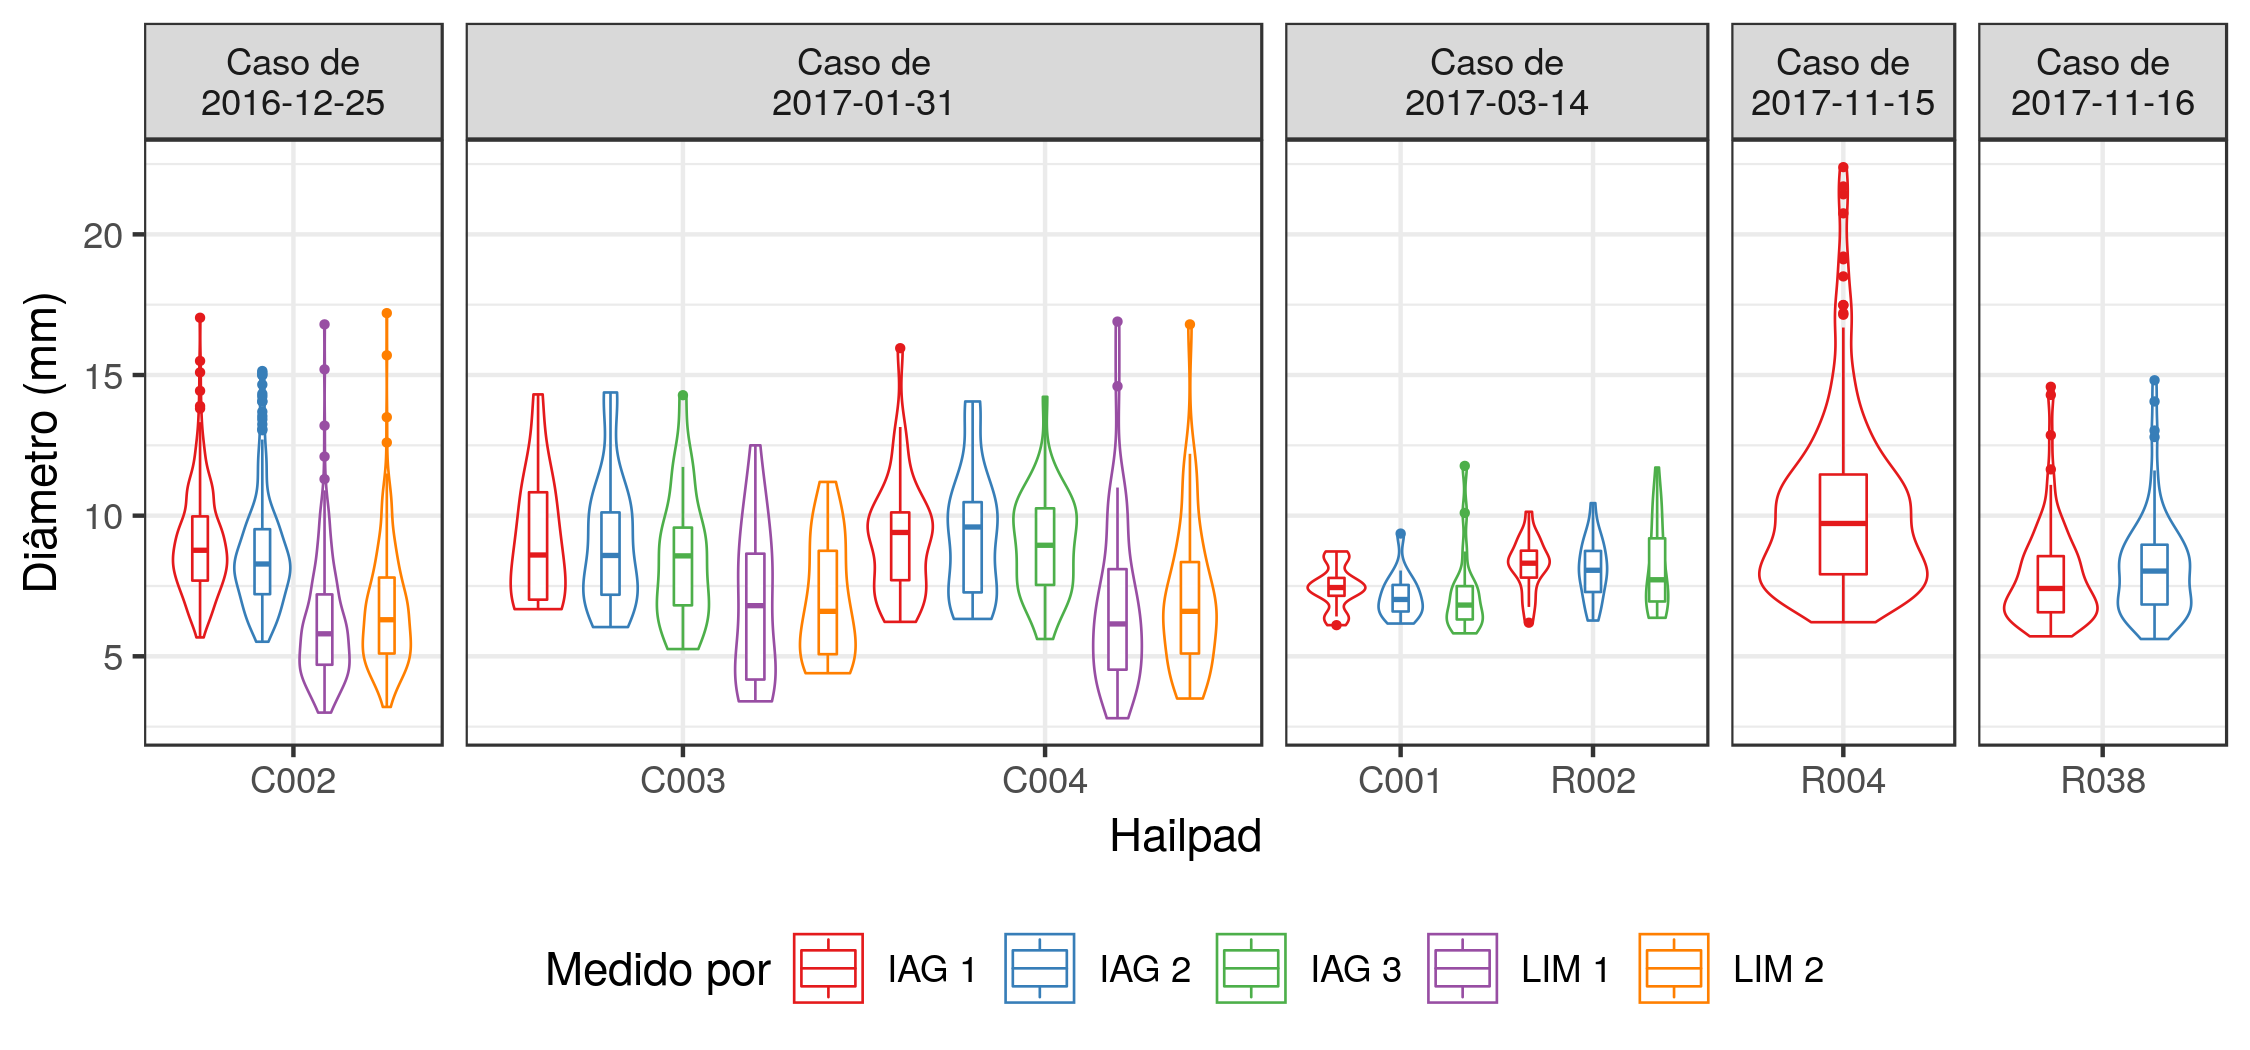
\includegraphics[width=\columnwidth]{../Hailpads_Processing/figures/measures_distribution_ptbr.png}
		\legend{Fonte: Produzido pela autora.}
	\end{center}
\end{figure}

Para os casos com medidas dos dois grupos (2016-12-25 e 2017-01-31), o IAG tende a medir diâmetros maiores que o LIM, que mede mais valores extremos principalmente no caso de 2016-12-25 (os diâmetros máximos de IAG 1, LIM 1 e LIM 2 são aproximadamente iguais). Já comparando as placas para um mesmo caso (2017-01-31 e 2017-03-14), as distribuições entre o primeiro e terceiro quartil são similares (no caso de 2017-01-31, por exemplo, as distribuições variaram entre $7$ e $10\:mm$ em todas as medidas do IAG nas duas placas), o que indica que o sistema convectivo que gerou a queda de granizo em um ponto não sofreu mudanças significativas quando gerou a queda de granizo no outro ponto. 

A \autoref{intensidade_anelfatorro} mostra a energia cinética de cada \textit{hailpad} em função do diâmetro do granizo para as escalas ANELFA e TORRO. As barras de erros mais largas em relação ao diâmetro são causadas pelo desvio-padrão maior em placas com maiores diferenças entre cada medida (\autoref{distribuicao_tamanho}). As duas escalas mostram resultados similares entre si, com a maioria das placas relacionadas a casos minimamente intensos porém defasados em relação aos índices mínimos: os diâmetros (máximos ou típicos) são equivalentes a um índice acima da energia cinética correspondente. Isso pode estar relacionado à \autoref{mezeix}, derivada a partir de medições de tempestades na Europa, assim como às próprias escalas que também foram estabelecidas a partir de tempestades no continente europeu: condições locais e sinóticas dessa região são distintas das condições da região de estudo, principalmente comparando sistemas de latitudes médias com tropicais, e essas condições são importantes na formação de granizo. \citeonline{Sanchez2009}, ao comparar distribuições de tamanho de granizo em três países com redes de \textit{hailpads}, mostram que podem ocorrer diferenças nos parâmetros característicos mesmos em localidades geograficamente próximas, diferença que pode ser propagada facilmente na estimativa da energia cinética dos \textit{hailpads}.

\begin{figure}[hbt]
	\begin{center}
		\caption{Energia cinética do \textit{hailpad} em função do diâmetro do granizo considerando as escalas ANELFA e TORRO, com os índices de A0 a A2 e de H0 a H2 (\autoref{tabela_escalas}) indicados} 
		\label{intensidade_anelfatorro}
		%		\setcaptionmargin{1cm}
		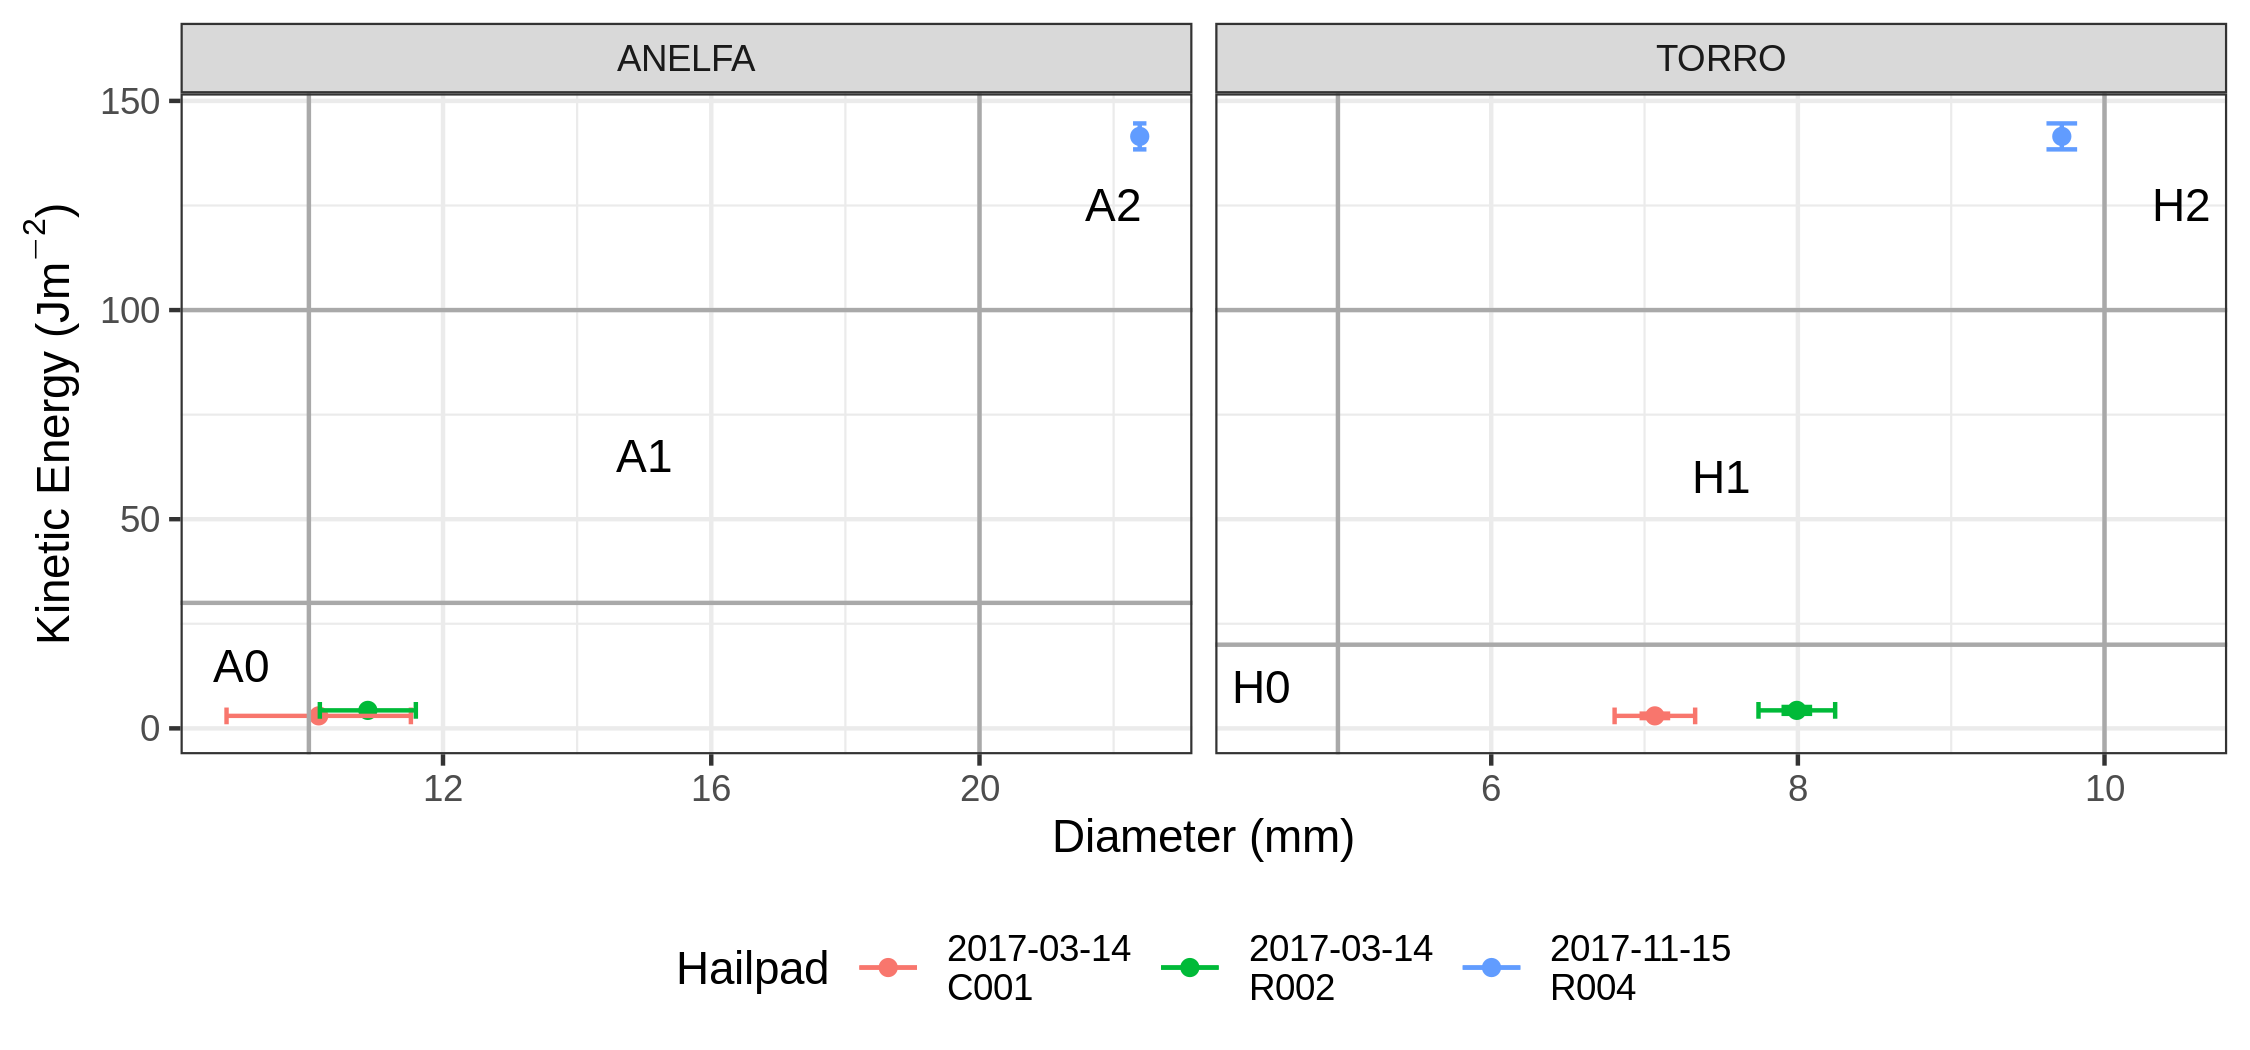
\includegraphics[width=\columnwidth]{../Hailpads_Processing/figures/data_anelfa_torro_ptbr.png}
		\legend{Fonte: Produzido pela autora.}
		\nota{A escala ANELFA leva em conta o diâmetro máximo medido no \textit{hailpad}, enquanto que a escala TORRO leva em conta o diâmetro típico da distribuição medida no \textit{hailpad}.}
	\end{center}
\end{figure}

Dentro da escala ANELFA (painel esquerdo da \autoref{intensidade_anelfatorro}), o caso de 2017-11-15 foi considerado o mais intenso, dentro do índice A2 (danos sérios a vegetais e árvores - foram reportados danos à plantações próximas da localização do \textit{hailpad} em Indaiatuba), com o caso de 2016-12-25 sendo o segundo mais intenso, dentro do índice A1 (danos à vinhas e pomares). No caso de 2017-03-14, com mais de um \textit{hailpad}, a queda de granizo em Indaiatuba (placa R002) foi ligeiramente mais intensa do que em Cosmópolis (placa C004) (diferença de $1\:mm$ no diâmetro máximo e de cerca de $2\:Jm^{-2}$ de energia cinética). Dentro da escala TORRO (painel direito da \autoref{intensidade_anelfatorro}) os resultados foram similares, com o caso de 2017-11-15 sendo o mais intenso também mas ligeiramente fora do índice H2 (tempestade significante) e o caso de 2016-12-25 sendo o segundo mais intenso, dentro do índice H1 (tempestade potencialmente prejudicial). A queda de granizo em Indaiatuba no caso de 2017-03-14 também foi ligeiramente mais intensa do que em Cosmópolis.

A \autoref{painel_ciclo} mostra a evolução temporal da refletividade máxima em $3\:km$ de altura (a), tamanho do sistema convectivo (b) e taxa de raios (c), enquanto que a \autoref{tabela_resumo_casos} mostra um panorama geral das características físicas relacionadas ao ciclo de vida dos casos em análise. De forma geral, a queda de granizo ocorreu dentro da fase de maturação dos sistemas convectivos, com refletividade acima de $60\:dBZ$, área em relativo crescimento e intensa atividade elétrica. O caso de 2017-01-31 foi o com menor tempo de vida ($0,5\:h$), área máxima ($69\:km^2$) e quantidade de raios ($8\:flashes$), mas não teve o menor tamanho de granizo: o caso de 2016-12-25 teve o menor granizo médio, enquanto que o caso de 2017-03-14 teve o menor granizo máximo (e granizo médio ligeiramente maior). O mesmo caso de 2017-03-14 foi o com maior tempo de vida ($6,2\:h$), refletividade máxima ($69,7\:dBZ$) e quantidade e taxa máxima de raios (15131 (4185) $flashes$ IC (CG), com taxa máxima de 125 (33) $flashes\:min^{-1}$ IC (CG)). Outro caso a ser destacado é o de 2017-11-15, com tempo de vida curto ($2,2\:h$), área máxima pequena ($253\:m^2$) e pouca quantidade de raios (menos de 200 $flashes$ somando IC e CG, taxa máxima abaixo de $10\:flashes\:min^{-1}$), mas que mostrou granizos acima de $10\:mm$ em média e granizo máximo de $22,4\:mm$. Considerando o papel do granizo na formação de raios (\autoref{granizo_eletrificacao}), é de se esperar uma relação direta entre mudança da atividade elétrica e queda de granizo (\autoref{painel_ciclo}c), porém ela não foi consistente em todos os casos: em 2016-12-25, 2017-03-14 e 2017-11-15 há um ligeiro aumento da atividade elétrica (principalmente raios IC) até 30 minutos antes da queda de granizo, enquanto que em 2017-01-31 não há raios suficientes para determinar aumento ou diminuição da atividade elétrica, e em 2017-11-16 há um aumento da atividade elétrica depois da queda de granizo.

\begin{figure}[hp]
	\begin{center}
		\caption{Evolução temporal da refletividade máxima em $3\:km$ (a), tamanho do sistema (b) e taxa de \textit{flashes} CG e IC (c). As linhas pontilhadas indicam o momento aproximado em que houve a queda de granizo medida no \textit{hailpad}} 
		\label{painel_ciclo}
		%		\setcaptionmargin{1cm}
		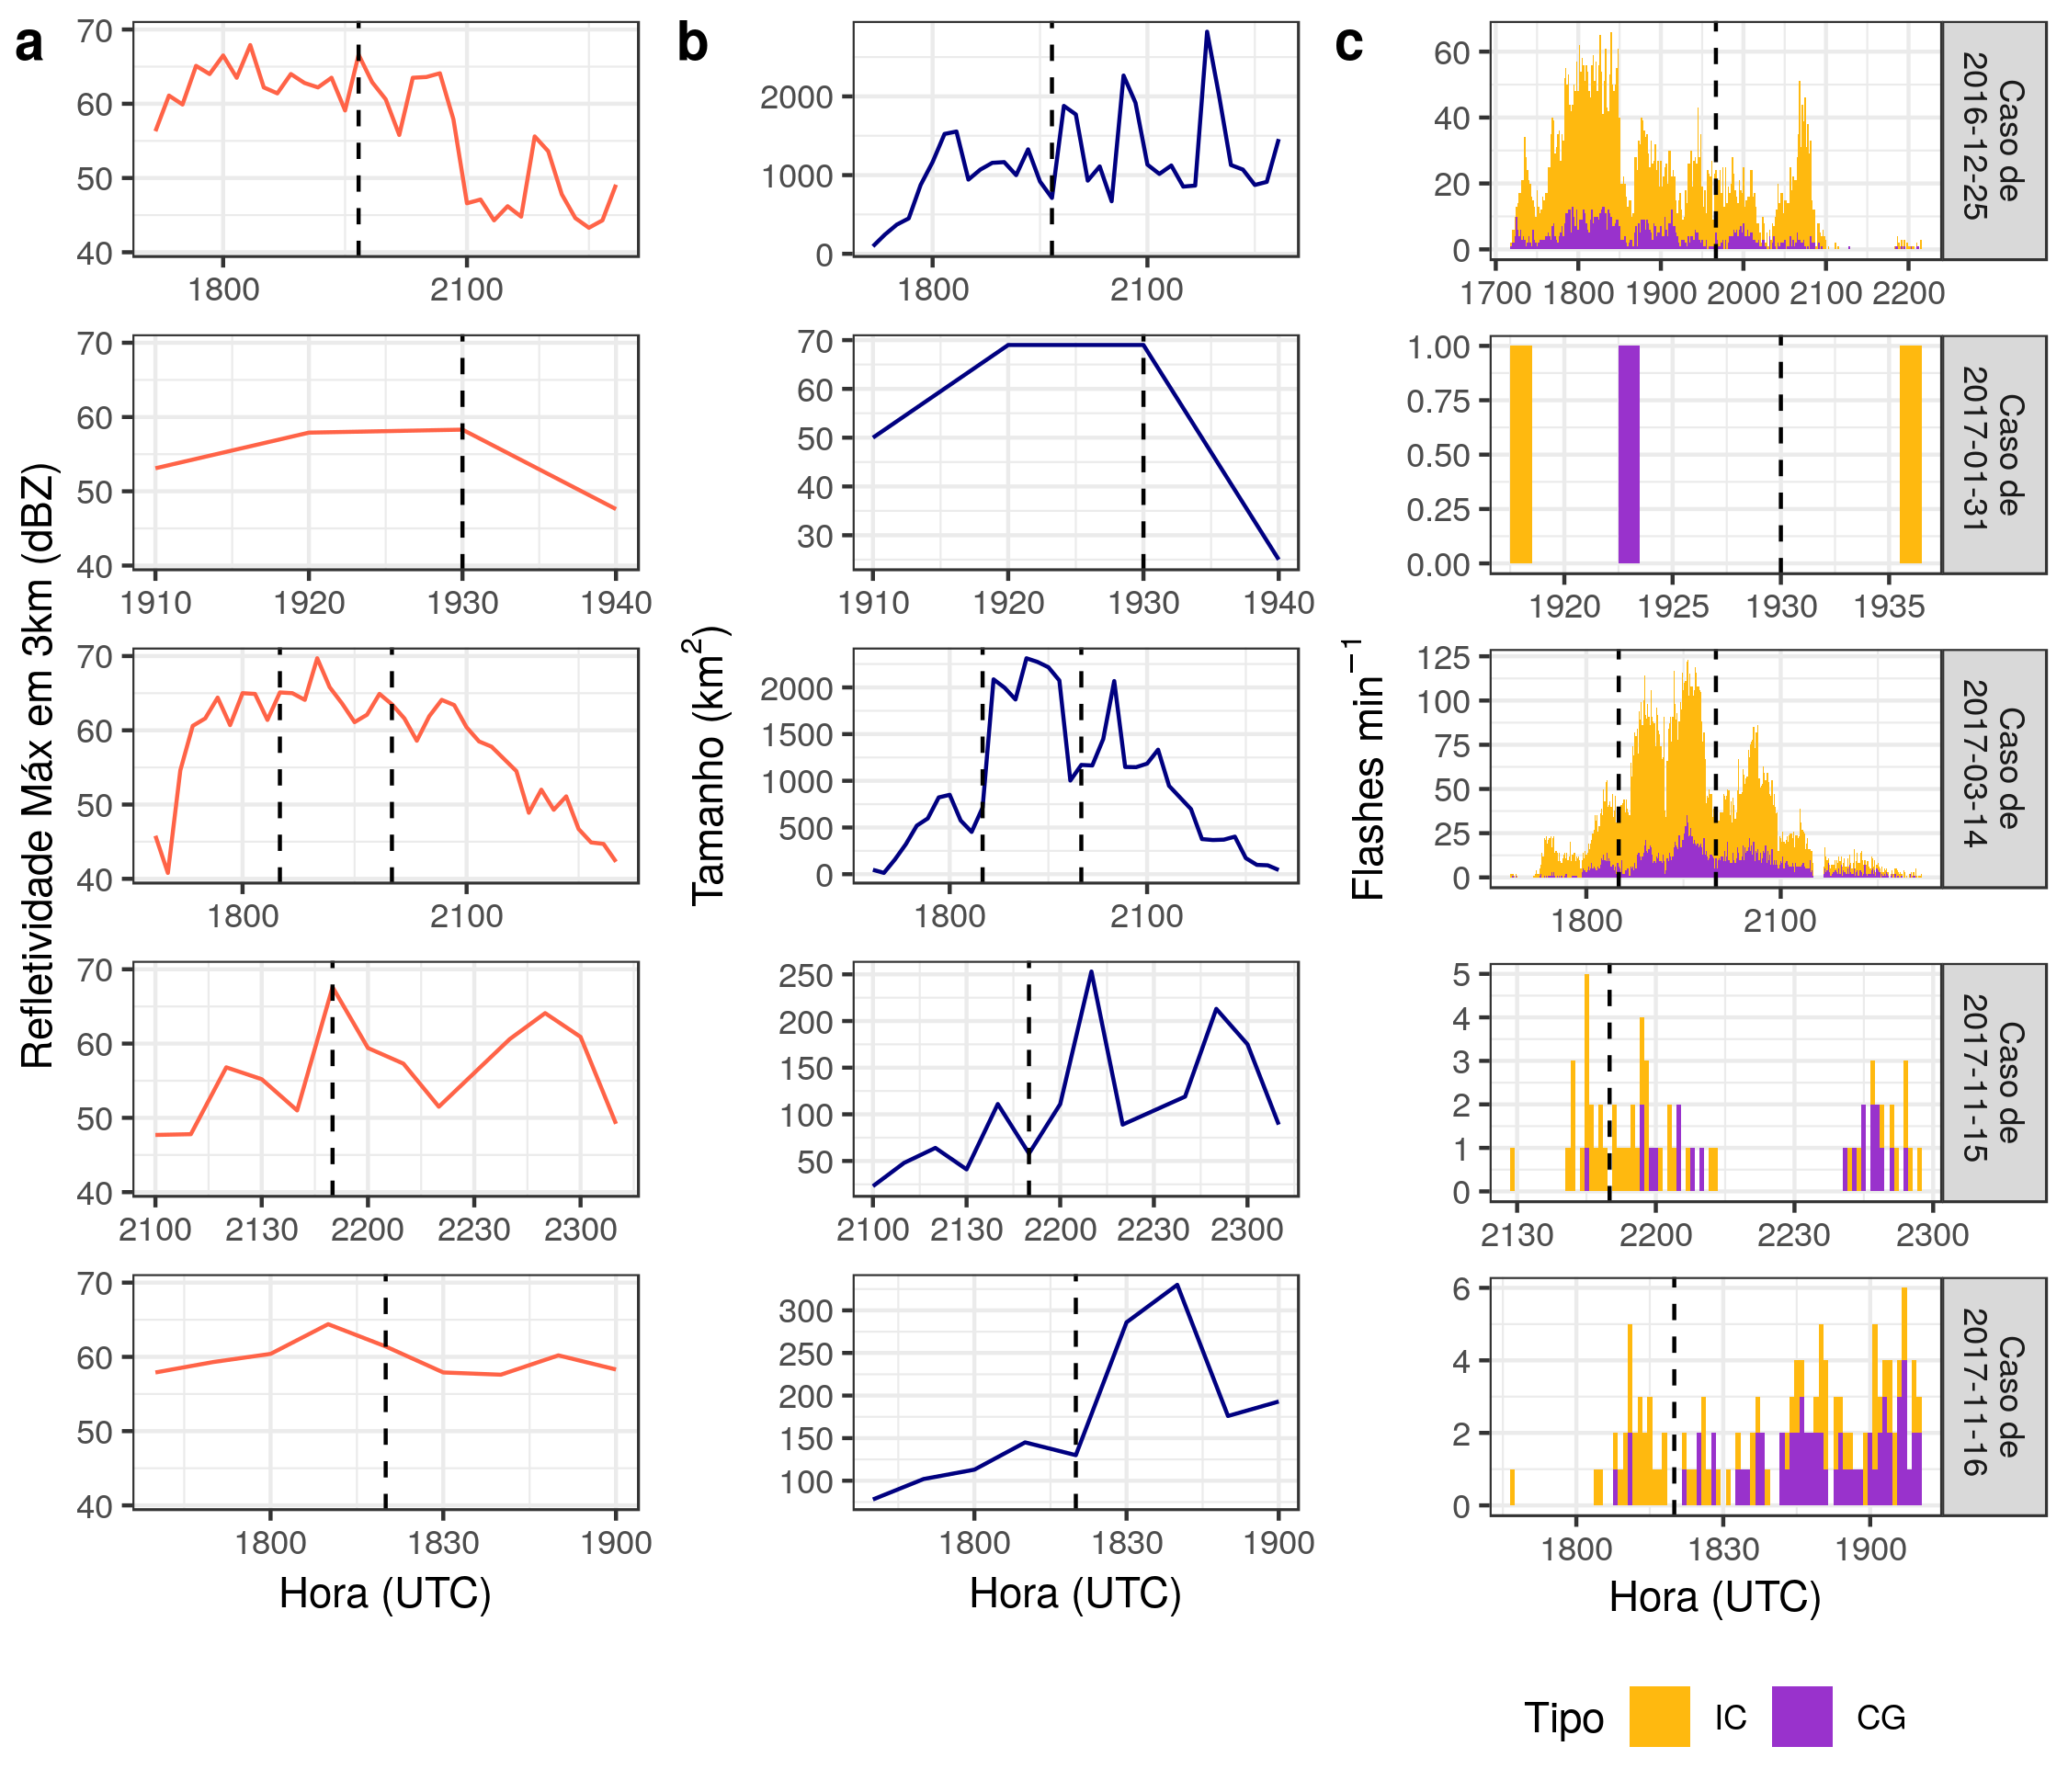
\includegraphics[width=0.99\columnwidth]{../General_Processing/figures/cases_dbz_size_lightning_ptbr.png}
		\legend{Fonte: Produzido pela autora.}
	\end{center}
\end{figure}

\begin{table}[htb]
	\IBGEtab{%
		\caption{Resumo das principais características físicas e elétricas dos casos analisados}%
		\label{tabela_resumo_casos}
	}{%
		\begin{tabularx}{\textwidth}{cY>{\hsize=1.5\hsize}Y>{\hsize=1.5\hsize}Y>{\hsize=1.5\hsize}Y>{\hsize=1.5\hsize}Y>{\hsize=0.75\hsize}Y>{\hsize=0.75\hsize}YYY}
			\toprule
			Caso & Tempo de Vida ($h$) & Z Máximo em $3\:km$ ($dBZ$) & Área Máxima ($km^2$) & Granizo Médio ($mm$) & Granizo Máximo ($mm$) & \multicolumn{2}{>{\hsize=2\hsize}Y}{Total de Raios ($flashes$)} & \multicolumn{2}{>{\hsize=2\hsize}Y}{Taxa Máxima de Raios ($flashes\ min^{-1}$)} \\
			\cmidrule(l){7-10}
			 & & & & & & IC & CG & IC & CG \\
			\midrule
			2016-12-25 & $5,7$ & $67,9$ & $2822$ & $7,6$ & $17,2$ & $13130$ & $2260$ & $104$ & $26$ \\
			\midrule 
			2017-01-31 & $0,5$ & $58,3$ & $69$ & $8,2$ & $16,9$ & $4$ & $4$ & $1$ & $1$ \\
			\midrule 
			2017-03-14 & $6,2$ & $69,7$ & $2312$ & $7,8$ & $11,8$ & $15131$ & $4185$ & $125$ & $33$ \\
			\midrule 
			2017-11-15 & $2,2$ & $67,6$ & $253$ & $10,3$ & $22,4$ & $86$ & $29$ & $8$ & $3$ \\
			\midrule 
			2017-11-16 & $1,3$ & $64,4$ & $330$ & $8$ & $14,8$ & $528$ & $227$ & $19$ & $8$ \\
			\bottomrule
		\end{tabularx}%
	}{%
		\fonte{Produzido pela autora.}%
	}
\end{table}


A partir dos resultados descritos nesta seção, dois casos foram escolhidos para uma análise mais detalhada:

\begin{alineas}
	\item \textbf{2017-03-14}: Classificado como tempestade com queda de granizo de baixa intensidade, este caso teve alta atividade elétrica durante seu longo ciclo de vida, gerando queda de granizo em dois pontos diferentes. Os dois momentos em que houve queda de granizo serão comparados em relação à estrutura e cinemática da nuvem;
	\item \textbf{2017-11-15}: Classificado com tempestade com queda de granizo de intensidade significativa, este caso teve baixa atividade elétrica, o que não é esperado em uma tempestade com produção de granizo suficiente para cair no solo com tamanho considerável. A microfísica e cinemática desta tempestade com ciclo de vida mais curto ajudará a explicar esse comportamento.
\end{alineas}

\section{Estudos de Caso}\label{estudo_casos}

Os estudos dos casos de 2017-03-14 e 2017-11-15 estão descritos a seguir, focando: no ambiente sinótico e termodinâmico em que os sistemas convectivos se formaram; na atividade elétrica ao longo dos ciclos de vida; na microfísica através da estrutura vertical da convecção quando houve queda de granizo e; na cinemática, observando os campos de vento derivado por Multi-Doppler antes e durante a queda de granizo.

\subsection{Caso de 2017-03-14}

\subsubsection{Ambiente Sinótico e Termodinâmico}\label{sinotica_201703014}

A influência de uma frente fria no litoral de São Paulo e do Rio de Janeiro durante a madrugada foi determinante para o disparo de sistemas convectivos no estado de São Paulo durante a tarde. O sistema frontal em si se deslocou para o Oceano Atlântico ao longo do dia - às 1200 UTC (Figura\autoref{era5_2017031412_jets}), o sistema está à leste de $30^{\circ}W$ - mas favoreceu a convergência de umidade na região de estudo (não mostrado). Às 1200 UTC, a radiossondagem (\autoref{sondagem_20170314}) mostra uma camada úmida entre a superfície e $600\:hPa$, mas com CAPE (\textit{Convective Available Potential Energy}, Energia Potencial Disponível para Convecção) nulo e pouco cisalhamento (mesma condição no resto do estado, como mostra a Figura\autoref{era5_2017031412_cape}). Já às 1500 UTC (Figura\autoref{era5_2017031415_cape}), o potencial para convecção (CAPE entre 500 e $1500\:J\:kg^{-1}$) e o cisalhamento (de até 10 nós) aumentaram, disparando sistemas convectivos no centro do estado de São Paulo. As imagens de satélite da \autoref{goes16_sp_20170314} mostram a propagação e intensificação de sistemas convectivos com topos de até $-75^{\circ}C$ de temperatura de brilho em alguns pontos na região de estudo aproximadamente às 1800 (a) e 2000 UTC (b), o que inclui o sistema que causou queda de granizo em Cosmópolis e Indaiatuba. 

\begin{figure}[htb]
	\begin{center}
		\caption{Campos da reanálise do ERA5 em 2017-03-14: Pressão ao nível médio do mar, espessura entre $1000$ e $500\:hPa$ e velocidade do vento em $250\:hPa$ às 1200 UTC (a); altura geopotencial em $850\:hPa$, cisalhamento do vento entre $1000$ e $500\:hPa$ e CAPE em superfície às 1200 (b) e 1500 UTC, no domínio do Estado de São Paulo (c)} 
		\label{era5_20170314_main}
		\subfloat[]{\includegraphics[width=0.5\columnwidth]{../Reanalysis_Processing/figures/ERA5_SA_sfc-jets_201703141200.png}
			\label{era5_2017031412_jets}}
		\subfloat[]{\includegraphics[width=0.5\columnwidth]{../Reanalysis_Processing/figures/ERA5_SA_cape-shear_2017031412.png}
			\label{era5_2017031412_cape}} \\
		\subfloat[]{\includegraphics[width=0.5\columnwidth]{../Reanalysis_Processing/figures/ERA5_SP-BR_cape-shear_2017031415.png}
			\label{era5_2017031415_cape}} \\
		\legend{Fonte: Produzido pela autora.}
	\end{center}
\end{figure}

\begin{figure}[hp]
	\begin{center}
		\caption{Plotagem Skew-T Log-P da radiossondagem do Campo de Marte (SP) com hodógrafa do vento e índices CAPE e CIN em 2017-03-14 1200 UTC.} 
		\label{sondagem_20170314}
		%		\setcaptionmargin{1cm}
		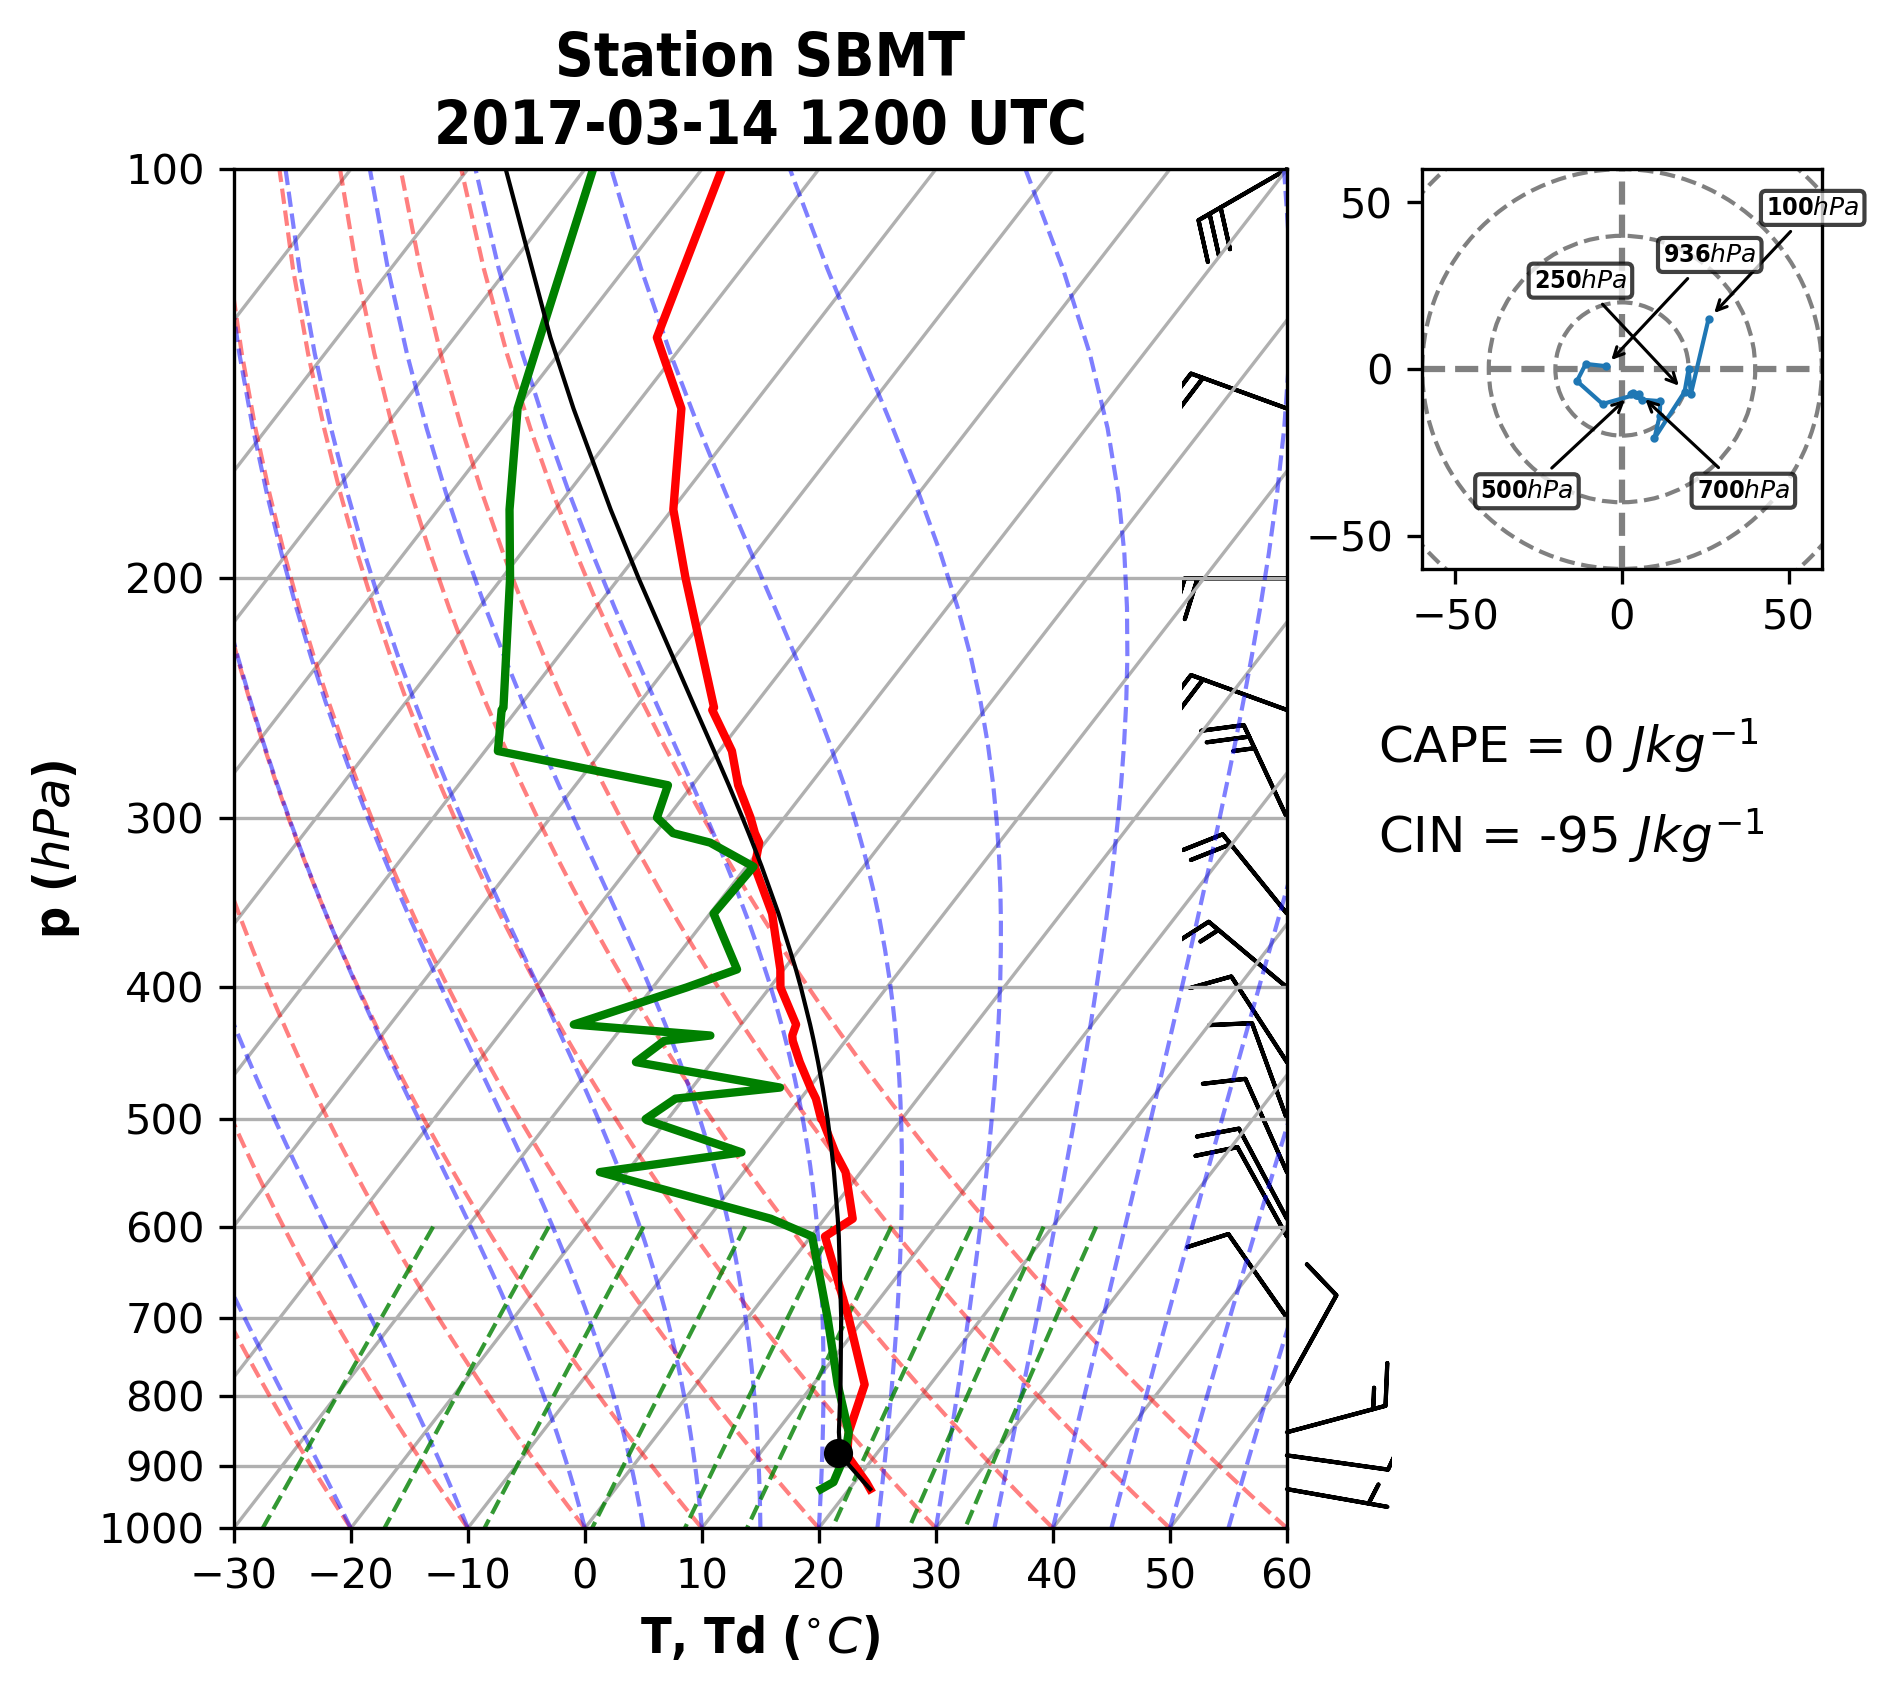
\includegraphics[width=0.75\columnwidth]{../Sounding_Processing/figures/sounding_SBMT2017031412UTC.png}
		\legend{Fonte: Produzido pela autora.}
	\end{center}
\end{figure}

%\begin{figure}[htb]
%	\begin{center}
%		\caption{Imagem de satélite do canal 13 do GOES-16 mostrando a temperatura de brilho do topo das nuvens na América do Sul em 2017-03-14 1751 UTC.} 
%		\label{goes16_sa_20170314}
%		%		\setcaptionmargin{1cm}
%		\includegraphics[width=0.75\columnwidth]{../Satellite_Processing/figures/Band_13/GOES16_B13_SA_SD201703141751.png}
%		\legend{Fonte: Produzido pela autora.}
%	\end{center}
%\end{figure}
%
\begin{figure}[hp]
	\begin{center}
		\caption{Imagem de satélite do canal 13 do GOES-16 mostrando a temperatura de brilho do topo das nuvens no estado de São Paulo em 2017-03-14 1751 (a) e 1951 UTC (b).} 
		\label{goes16_sp_20170314}
		\subfloat[]{\includegraphics[width=0.5\columnwidth]{../Satellite_Processing/figures/Band_13/GOES16_B13_SP-BR_SD201703141751.png}
			\label{goes16_sp_20170314_1}}
		\subfloat[]{\includegraphics[width=0.5\columnwidth]{../Satellite_Processing/figures/Band_13/GOES16_B13_SP-BR_SD201703141951.png}
			\label{goes16_sp_20170314_2}} \\
		\legend{Fonte: Produzido pela autora.}
	\end{center}
\end{figure}

\subsubsection{Eletrificação}\label{elec_201703014}

A \autoref{track_flashes_20170314} mostra a localização do sistema ao longo do ciclo de vida e dos \textit{flashes} associados a ele. Como já mostrado (\autoref{painel_ciclo}, \autoref{tabela_casos}), este caso teve um longo ciclo de vida com intensa atividade elétrica - a taxa de \textit{flashes} chega a um máximo (125 (33) $flashes\:\:min^{-1}$ IC (CG)) após a queda de granizo em Cosmópolis e diminui antes do evento em Indaiatuba. O sistema convectivo se deslocou por toda a RMC e regiões vizinhas na direção sudoeste, com fusões e separações com sistemas menores. Os \textit{flashes} IC e CG ocorreram principalmente dentro da RMC durante todo o ciclo de vida, com cerca de 10 vezes mais \textit{flashes} IC do que CG.

\begin{figure}[htb]
	\begin{center}
		\caption{Rastreamento (a) e localização dos \textit{flashes} IC e CG (b) do sistema convectivo responsável pelas quedas de granizo em Cosmópolis e Indaiatuba em 2017-03-14. Os triângulos pretos indicam a localização dos \textit{hailpads}.} 
		\label{track_flashes_20170314}
		%		\setcaptionmargin{1cm}
		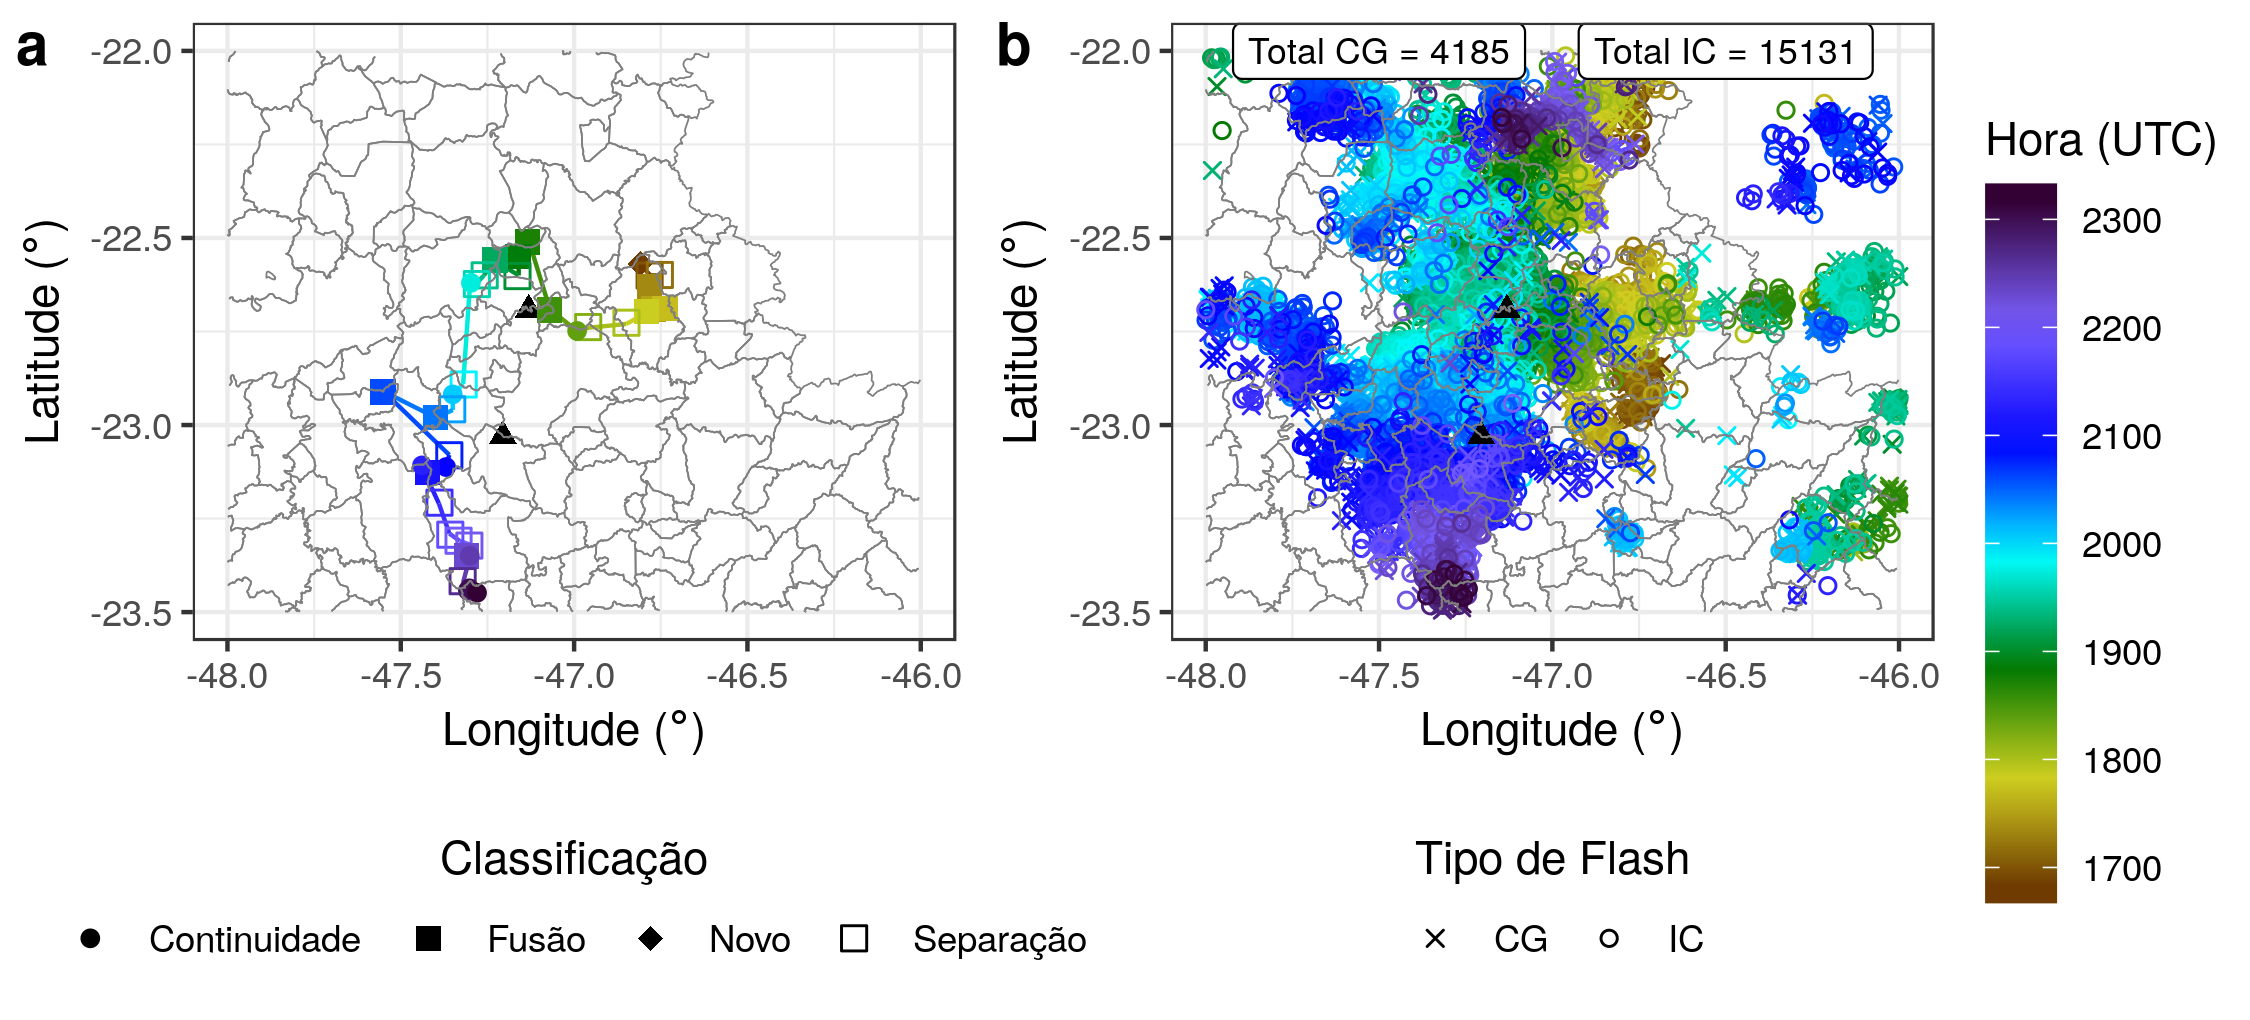
\includegraphics[width=\columnwidth]{../General_Processing/figures/track_flashes_20170314_ptbr.png}
		\legend{Fonte: Produzido pela autora.}
	\end{center}
\end{figure}

\subsubsection{Microfísica}\label{micro_201703014}

A \autoref{radar_20170314_1} mostra os campos de refletividade e variáveis polarimétricas refletividade diferencial, fase diferencial específica e coeficiente de correlação do radar da FCTH para o caso de 2017-03-14, quando houve queda de granizo em Cosmópolis; a \autoref{radar_derived_20170314_1} mostra a identificação de hidrometeoros e massas de água líquida e gelo calculadas a partir dos campos de radar. O núcleo convectivo que causou a queda de granizo está embebido em um sistema multicelular que abrange boa parte da RMC. Esse núcleo é formado por uma região de refletividade acima de $50\:dBZ$ de cerca de $10\:km$ de extensão horizontal e vertical (da superfície até a isoterma de $-40\:^{\circ}C$) (\autoref{radar_20170314_1}a). Os valores abaixo de 0,9 de coeficiente de correlação entre a superfície e a isoterma de $0\:^{\circ}C$ (\autoref{radar_20170314_1}d) confirmam a presença de granizo ou a coexistência de granizo e chuva em vez de apenas chuva (também associado a altas refletividades) nessa região.

Os campos derivados das variáveis polarimétricas são acurados na classificação de granizo no núcleo convectivo responsável pela queda de granizo em Cosmópolis (\autoref{radar_derived_20170314_1}a) e na massa de gelo associada (que chegou a cerca de $15\:gm^{-3}$ próximo à superfície, \autoref{radar_derived_20170314_1}c), mas apresentam problemas em outros aspectos. A classificação de hidrometeoros é muito similar ao campo de refletividade, com regiões de refletividade acima de $50\:dBZ$ classificadas como granizo, entre 40 e $50\:dBZ$ como graupel de densidade alta e entre 30 e $40\:dBZ$ como graupel de densidade baixa; o problema está em regiões com refletividade abaixo de $30\:dBZ$ classificadas como cristais de gelo e agregados, mesmo abaixo da isoterma de $0\:^{\circ}C$ (gelo vertical próximo à superfície em $\ang{22.79}S$, $\ang{47.24}W$, por exemplo), condição muito difícil de ser encontrada em nuvens frias de tempestades tropicais. É importante ressaltar que a mesma radiossondagem que foi usada para delimitar as isotermas de 0 e $-40\:^{\circ}C$ serviu de entrada para o algoritmo de identificação de hidrometeoros, mas possivelmente a ponderação dada para essa variável foi insuficiente, assim como para as outras variáveis polarimétricas (no mesmo exemplo de gelo vertical próximo à superfície, a refletividade diferencial (\autoref{radar_20170314_1}b) é acima do valor que indica esse hidrometeoro (\autoref{hid_straka}b)). O campo de massa de água líquida (\autoref{radar_derived_20170314_1}b) apresenta o mesmo problema, onde é possível observar massa de $1\:gm^{-3}$ acima da isoterma de $-40\:^{\circ}C$ no núcleo associado à queda de granizo; mesmo sendo um valor baixo, é difícil encontrar água na forma líquida em regiões com temperaturas tão baixas.

\begin{figure}[hp]
	\centering
	\caption{Corte horizontal em $3\:km$ de altura e vertical entre os pontos A e B de campos do radar da FCTH em 2017-03-14 1827 UTC, quando houve queda de granizo em Cosmópolis: Refletividade corrigida (a) e diferencial (b), fase diferencial específica (c) e coeficiente de correlação (d). O 'x' indica a localização do \textit{hailpad} e as isotermas de $0$ e $-40^{\circ}C$ foram definidas a partir da radiossondagem de SMBT}
	\label{radar_20170314_1}
	\vspace{-5pt}
	\includegraphics[width=\columnwidth]{../Radar_Processing/figures/ppis/classification/FCTH Corrected Reflectivity 2017-03-14 1827 UTC.png} \\
	\vspace{-5pt}
	\includegraphics[width=\columnwidth]{../Radar_Processing/figures/ppis/classification/FCTH Differential Reflectivity 2017-03-14 1827 UTC.png} \\
	\vspace{-5pt}
	\includegraphics[width=\columnwidth]{../Radar_Processing/figures/ppis/classification/FCTH Specific Differential Phase 2017-03-14 1827 UTC.png} \\
	\vspace{-5pt}
	\includegraphics[width=\columnwidth]{../Radar_Processing/figures/ppis/classification/FCTH Cross Correlation Ratio 2017-03-14 1827 UTC.png} \\
	\legend{Fonte: Produzido pela autora.}
\end{figure}

\begin{figure}[hp]
	\centering
	\caption{Corte horizontal em $3\:km$ de altura e vertical entre os pontos A e B de campos derivados do radar da FCTH em 2017-03-14 1827 UTC, quando houve queda de granizo em Cosmópolis: Identificação de hidrometeoros (a) e massas de água líquida (b) e gelo (c). O 'x' indica a localização do \textit{hailpad} e as isotermas de $0$ e $-40^{\circ}C$ foram definidas a partir da radiossondagem de SMBT} 
	\label{radar_derived_20170314_1}
	\vspace{-5pt}
	\includegraphics[width=\columnwidth]{../Radar_Processing/figures/ppis/classification/FCTH Hydrometeor ID 2017-03-14 1827 UTC.png} \\
	\vspace{-5pt}
	\includegraphics[width=\columnwidth]{../Radar_Processing/figures/ppis/classification/FCTH Liquid Water Mass 2017-03-14 1827 UTC.png} \\
	\vspace{-5pt}
	\includegraphics[width=\columnwidth]{../Radar_Processing/figures/ppis/classification/FCTH Ice Water Mass 2017-03-14 1827 UTC.png} \\
	\legend{Fonte: Produzido pela autora.}
\end{figure}

Depois da queda de granizo em Cosmópolis, o sistema convectivo se separou em diversos sistemas menores; o maior desses sistemas se intensificou e prosseguiu na direção sul/sudeste (\autoref{track_flashes_20170314}a), causando a queda de granizo em Indaiatuba. A \autoref{radar_20170314_2} mostra os campos de refletividade e variáveis polarimétricas do radar da FCTH para o caso de 2017-03-14, quando houve a queda de granizo; a \autoref{radar_derived_20170314_2} mostra a identificação de hidrometeoros e massas de água líquida e gelo calculadas a partir dos campos de radar. O núcleo convectivo responsável pela queda de granizo não é tão intenso quanto o de Cosmópolis, embebido em um sistema mais homogêneo que o anterior no oeste da RMC. Este núcleo tem valores de refletividade acima de $50\:dBZ$ em cerca de $12\:km$ de extensão horizontal, da superfície até a isoterma de $-40\:^{\circ}C$ (\autoref{radar_20170314_2}a). Os valores de fase diferencial específica acima de $1\:^{\circ}km^{-1}$ nessa região, entre a superfície e a isoterma de $0\:^{\circ}C$, confirmam a presença de chuva com gotas grandes e granizo (\autoref{radar_20170314_2}c).

A classificação de hidrometeoros do sistema convectivo que causou queda de granizo em Indaiatuba (\autoref{radar_derived_20170314_2}a) novamente é muito similar ao campo de refletividade, com granizo e gotas grandes próximo à superfície e granizo até a isoterma de $-40\:^{\circ}C$, na mesma região de refletividade acima de $50\:dBZ$; há também problemas com a identificação de agregados e cristais de gelo abaixo da isoterma de $0\:^{\circ}C$, associados à refletividades abaixo de $30\:dBZ$ (próximo aos pontos A e B, por exemplo, há uma camada de agregados entre a superfície e $4\:km$ de altura, incompatível com as variáveis polarimétricas). Em relação à massa de água líquida (\autoref{radar_derived_20170314_2}b), ela ficou limitada ao núcleo convectivo, com concentrações de até $5\:gm^{-3}$ próximo à superfície e abaixo da isoterma de $-40\:^{\circ}C$; a massa de gelo (\autoref{radar_derived_20170314_2}c) também ficou limitada ao núcleo convectivo, com concentrações de até $15\:gm^{-3}$ próximo à superfície.

\begin{figure}[hp]
	\centering
	\caption{Corte horizontal em $3\:km$ de altura e vertical entre os pontos A e B de campos do radar da FCTH em 2017-03-14 1957 UTC, quando houve queda de granizo em Indaiatuba: Refletividade corrigida (a) e diferencial (b), fase diferencial específica (c) e coeficiente de correlação (d). O 'x' indica a localização do \textit{hailpad} e as isotermas de $0$ e $-40^{\circ}C$ foram definidas a partir da radiossondagem de SMBT}
	\label{radar_20170314_2}
	\vspace{-5pt}
	\includegraphics[width=\columnwidth]{../Radar_Processing/figures/ppis/classification/FCTH Corrected Reflectivity 2017-03-14 1957 UTC.png} \\
	\vspace{-5pt}
	\includegraphics[width=\columnwidth]{../Radar_Processing/figures/ppis/classification/FCTH Differential Reflectivity 2017-03-14 1957 UTC.png} \\
	\vspace{-5pt}
	\includegraphics[width=\columnwidth]{../Radar_Processing/figures/ppis/classification/FCTH Specific Differential Phase 2017-03-14 1957 UTC.png} \\
	\vspace{-5pt}
	\includegraphics[width=\columnwidth]{../Radar_Processing/figures/ppis/classification/FCTH Cross Correlation Ratio 2017-03-14 1957 UTC.png} \\
	\legend{Fonte: Produzido pela autora.}
\end{figure}

\begin{figure}[htb]
	\centering
	\caption{Corte horizontal em $3\:km$ de altura e vertical entre os pontos A e B de campos derivados do radar da FCTH em 2017-03-14 1957 UTC, quando houve queda de granizo em Indaiatuba: Identificação de hidrometeoros (a) e massas de água líquida (b) e gelo (c). O 'x' indica a localização do \textit{hailpad} e as isotermas de $0$ e $-40^{\circ}C$ foram definidas a partir da radiossondagem de SMBT} 
	\label{radar_derived_20170314_2}
	\vspace{-5pt}
	\includegraphics[width=\columnwidth]{../Radar_Processing/figures/ppis/classification/FCTH Hydrometeor ID 2017-03-14 1957 UTC.png} \\
	\vspace{-5pt}
	\includegraphics[width=\columnwidth]{../Radar_Processing/figures/ppis/classification/FCTH Liquid Water Mass 2017-03-14 1957 UTC.png} \\
	\vspace{-5pt}
	\includegraphics[width=\columnwidth]{../Radar_Processing/figures/ppis/classification/FCTH Ice Water Mass 2017-03-14 1957 UTC.png} \\
	\legend{Fonte: Produzido pela autora.}
\end{figure}

\pagebreak

\subsubsection{Cinemática}\label{cinematica_201703014}

A \autoref{doppler_20170314_1} mostra os campos de refletividade mesclada e velocidade do vento derivado por Dual-Doppler usando a combinação dos radares de São Roque e FCTH, para o caso de 2017-03-14, quando houve queda de granizo em Cosmópolis. O sistema convectivo responsável pelo evento apresenta diversos núcleos convectivos com refletividade acima de $40\:dBZ$, sendo que o mais intenso deles está mais próximo à localização do \textit{hailpad}. Dez minutos antes da queda de granizo (1820 UTC - \autoref{doppler_20170314_1}a), esse núcleo principal tem cerca de $10\:km$ de extensão horizontal e $15\:km$ de altura, com refletividades acima de $50\:dBZ$ até $12\:km$ de altura. Uma região de corrente ascendente de $30\:ms^{-1}$ encontra-se acima da isoterma de $-40^{\circ}C$, com um escoamento ascendente entre 3 e $19\:km$ de altura, divergência no topo, e um escoamento descendente menos intenso entre 5 e $12\:km$. Às 1830 UTC (\autoref{doppler_20170314_2}b), o núcleo convectivo menos intenso à sudoeste do núcleo principal se intensifica e eles começam a se juntar. A região de corrente ascendente é mais fraca (cerca de $20\:ms^{-1}$) com a mesma extensão vertical, mas a intensificação do núcleo convectivo menor expande o escoamento ascendente horizontalmente, com um escoamento descendente ainda menos intenso fora do sistema convectivo. Próximo à localização do \textit{hailpad} (\autoref{doppler_20170314_2}b), a corrente ascendente é fraca (praticamente nula em alguns pontos) entre as isotermas de 0 e $-40^{\circ}C$, o que pode indicar a precipitação de hidrometeoros, incluindo granizo pequeno, como observado pelo \textit{hailpad} (\autoref{tabela_resumo_casos}).

\begin{figure}[htb]
	\centering
	\caption{Corte horizontal em $3\:km$ de altura e vertical entre os pontos A e B de refletividade e velocidade do vento (correntes ascendentes e descendentes máximas no painel da esquerda, escoamento no painel da direita) derivado por Multi-Doppler em 2017-03-14 às 1820 (a) e 1830 UTC (b), quando houve queda de granizo em Cosmópolis. O 'x' indica a localização do \textit{hailpad} e as isotermas de $0$ e $-40^{\circ}C$ foram definidas a partir da radiossondagem de SMBT} 
	\label{doppler_20170314_1}
	\vspace{-5pt}
	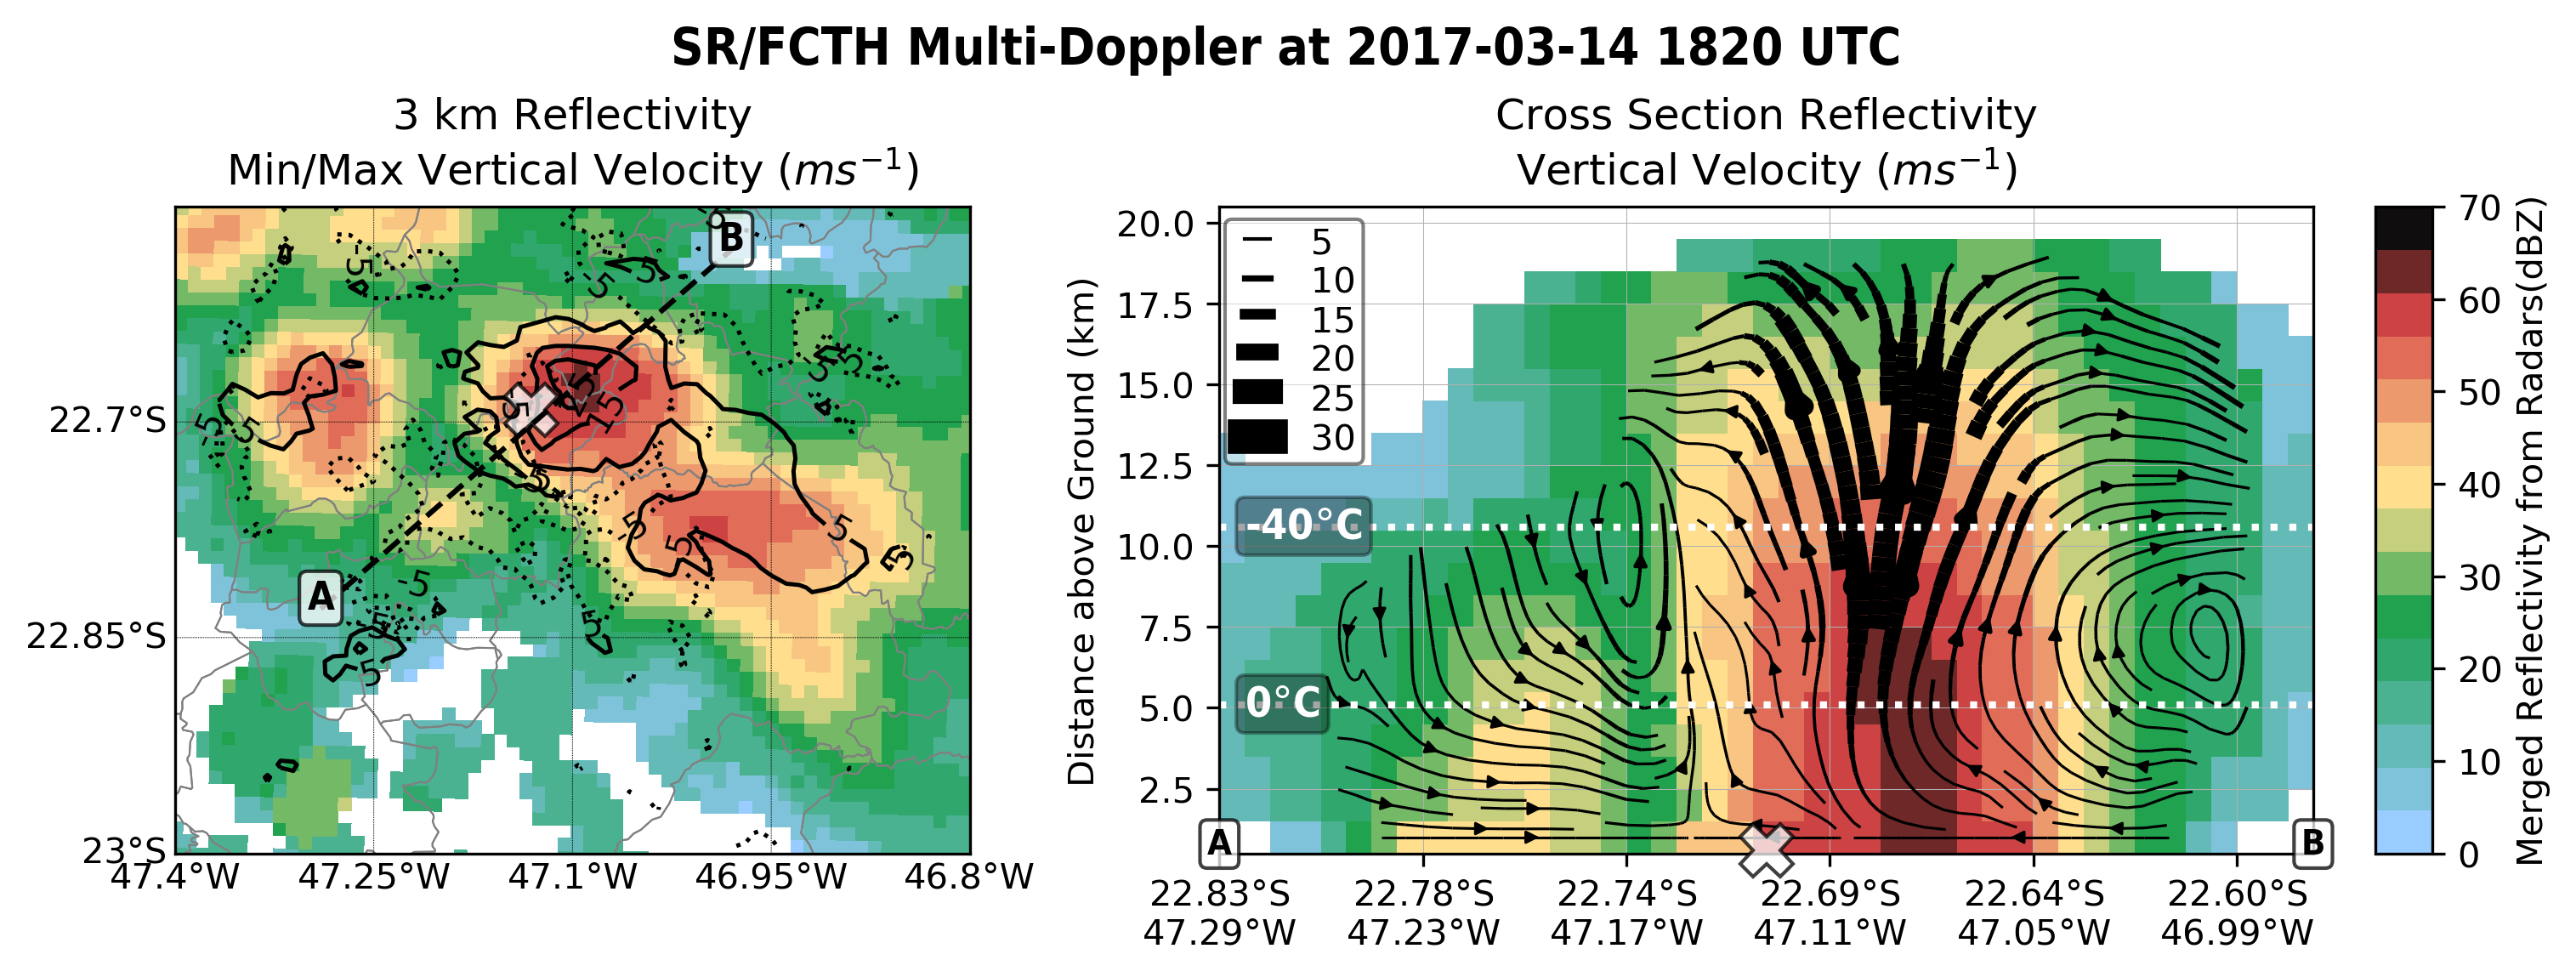
\includegraphics[width=\columnwidth]{../MultiDoppler_Processing/figures/SR-FCTH 2017-03-14 1820 UTC.png} \\
	\vspace{-5pt}
	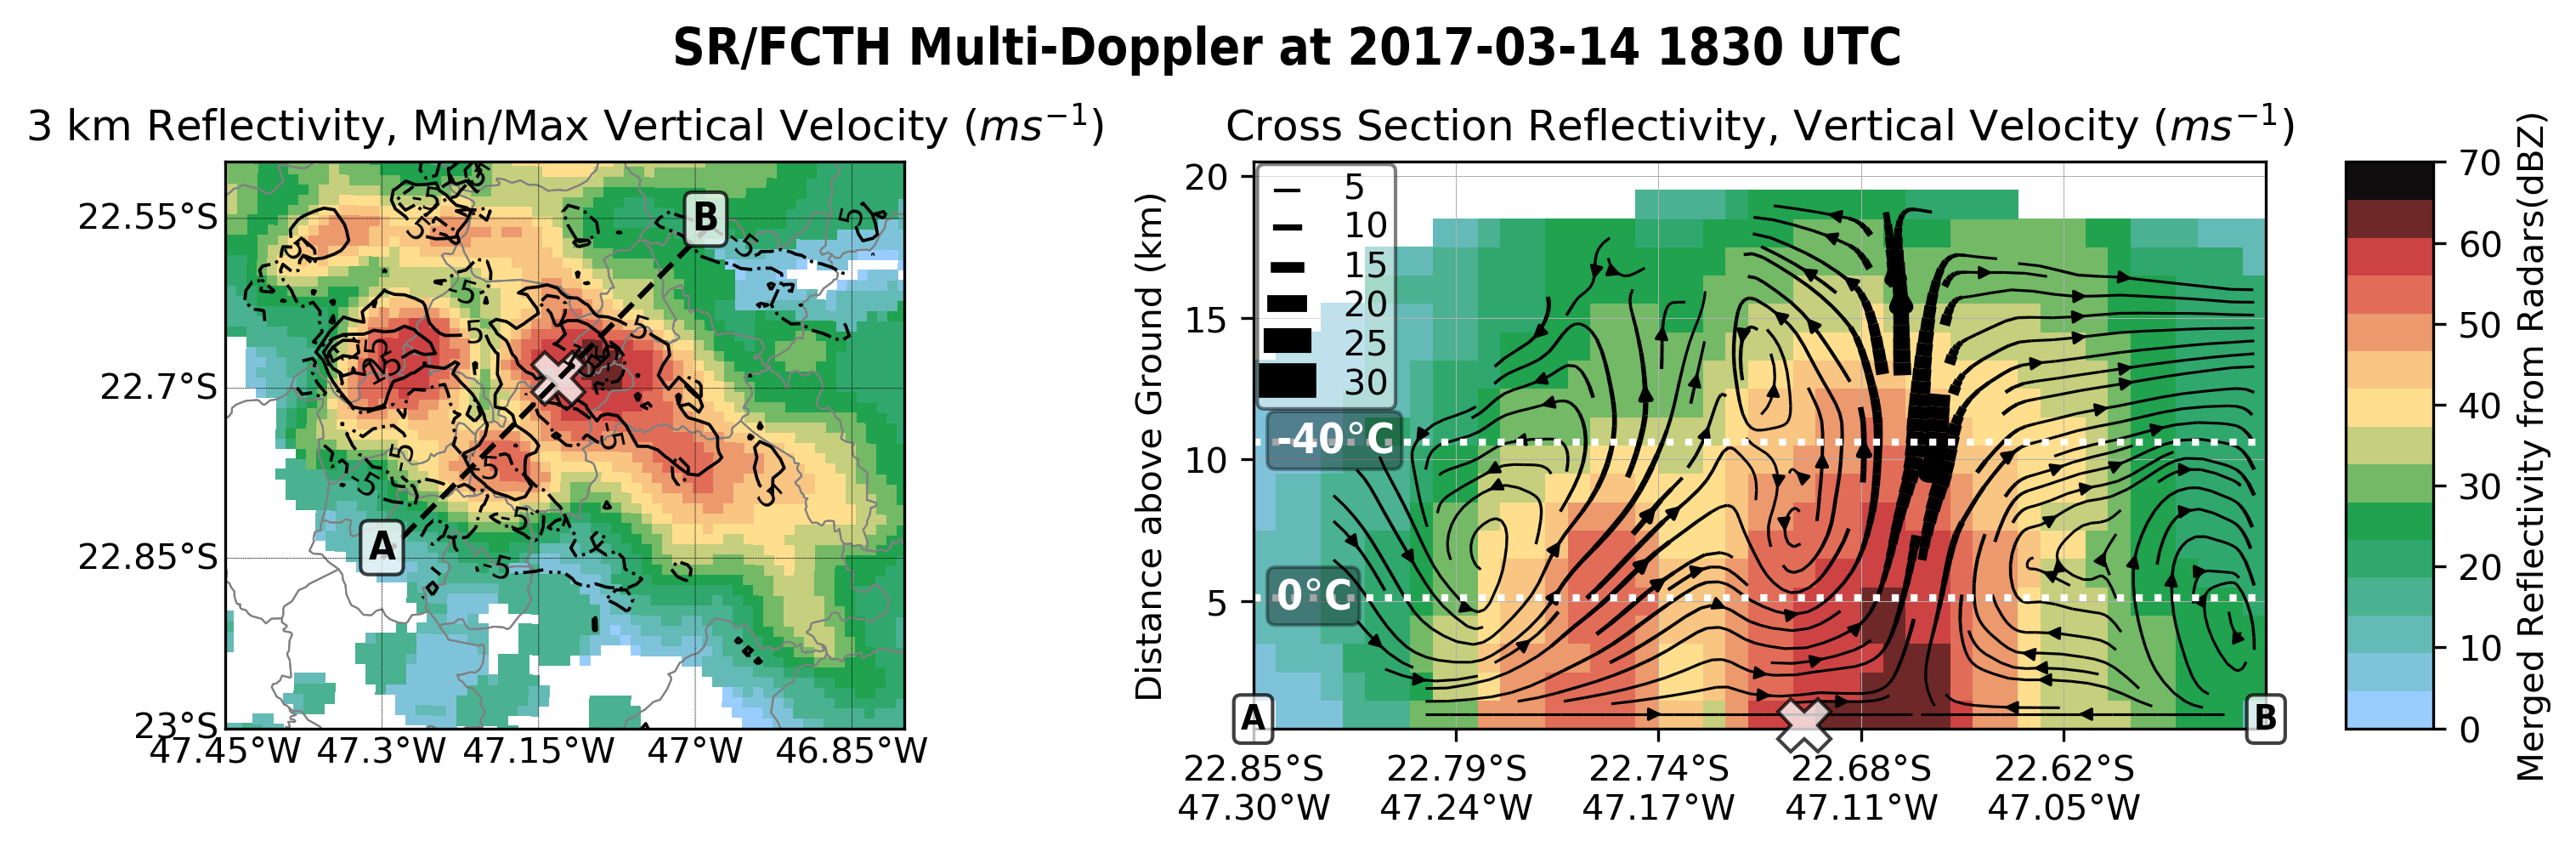
\includegraphics[width=\columnwidth]{../MultiDoppler_Processing/figures/SR-FCTH 2017-03-14 1830 UTC.png} \\
	\legend{Fonte: Produzido pela autora.}
\end{figure}

A \autoref{doppler_20170314_2} mostra os campos de refletividade mesclada e velocidade do vento derivada por Dual-Doppler para o caso de 2017-03-14, quando houve queda de granizo em Indaiatuba. Esta nova célula convectiva também possui um núcleo principal com refletividades acima de $40\:dBZ$, mas agora com maior extensão horizontal (cerca de $60\:km$ na direção noroeste-sudeste) e alguns picos de refletividade (acima de $55\:dBZ$) distintos, incluindo um próximo à localização do \textit{hailpad} (\autoref{doppler_20170314_2}a, painel da esquerda). Esse pico próximo ao \textit{hailpad} é associado a um núcleo de $15\:km$ de altura, com refletividade acima de $50\:dBZ$ até $12\:km$ de altura. Entre 1950 (\autoref{doppler_20170314_2}a) e 2000 UTC (\autoref{doppler_20170314_2}b), esse núcleo enfraquece (refletividade máxima e extensão vertical diminuem) ao mesmo tempo em que a área convectiva expande horizontalmente ao fundir com um sistema menor à oeste. Antes da queda de granizo (\autoref{doppler_20170314_2}a), algumas regiões de corrente ascendente de até $15\:ms^{-1}$ estão localizadas entre as isotermas de 0 e $-40^{\circ}C$ associadas com os picos de refletividade (55 a $60\:dBZ$), mas o escoamento ascendente não é bem definido, mostrando um escoamento horizontal acima de $15\:km$ e algumas regiões de correntes descendentes (de até $5\:ms^{-1}$); o escoamento descendente principal ocorre fora do núcleo convectivo. Dez minutos depois (\autoref{doppler_20170314_2}b), a região de corrente ascendente principal ($\ang{23.07}S$, $\ang{47.20}W$) se intensifica, com velocidade de até $25\:ms^{-1}$ e um escoamento ascendente bem definido entre 2 e $12\:km$ de altura; acima dessa região, a corrente descendente é mais fraca e o escoamento descendente principal ocorre fora do núcleo convectivo. Próximo à localização do \textit{hailpad}, a corrente ascendente é mais fraca entre as isotermas de 0 e $-40^{\circ}C$ e praticamente nula abaixo dessa região, indicando a precipitação de hidrometeoros, incluindo chuva e granizo pequeno, como observado pelo \textit{hailpad} (\autoref{tabela_resumo_casos}).

\begin{figure}[hbt]
	\centering
	\caption{Corte horizontal em $3\:km$ de altura e vertical entre os pontos A e B de refletividade e velocidade do vento (correntes ascendentes e descendentes máximas no painel da esquerda, escoamento no painel da direita) derivado por Multi-Doppler em 2017-03-14 às 1950 (a) e 2000 UTC (b), quando houve queda de granizo em Indaiatuba. O 'x' indica a localização do \textit{hailpad} e as isotermas de $0$ e $-40^{\circ}C$ foram definidas a partir da radiossondagem de SMBT} 
	\label{doppler_20170314_2}
	\vspace{-5pt}
	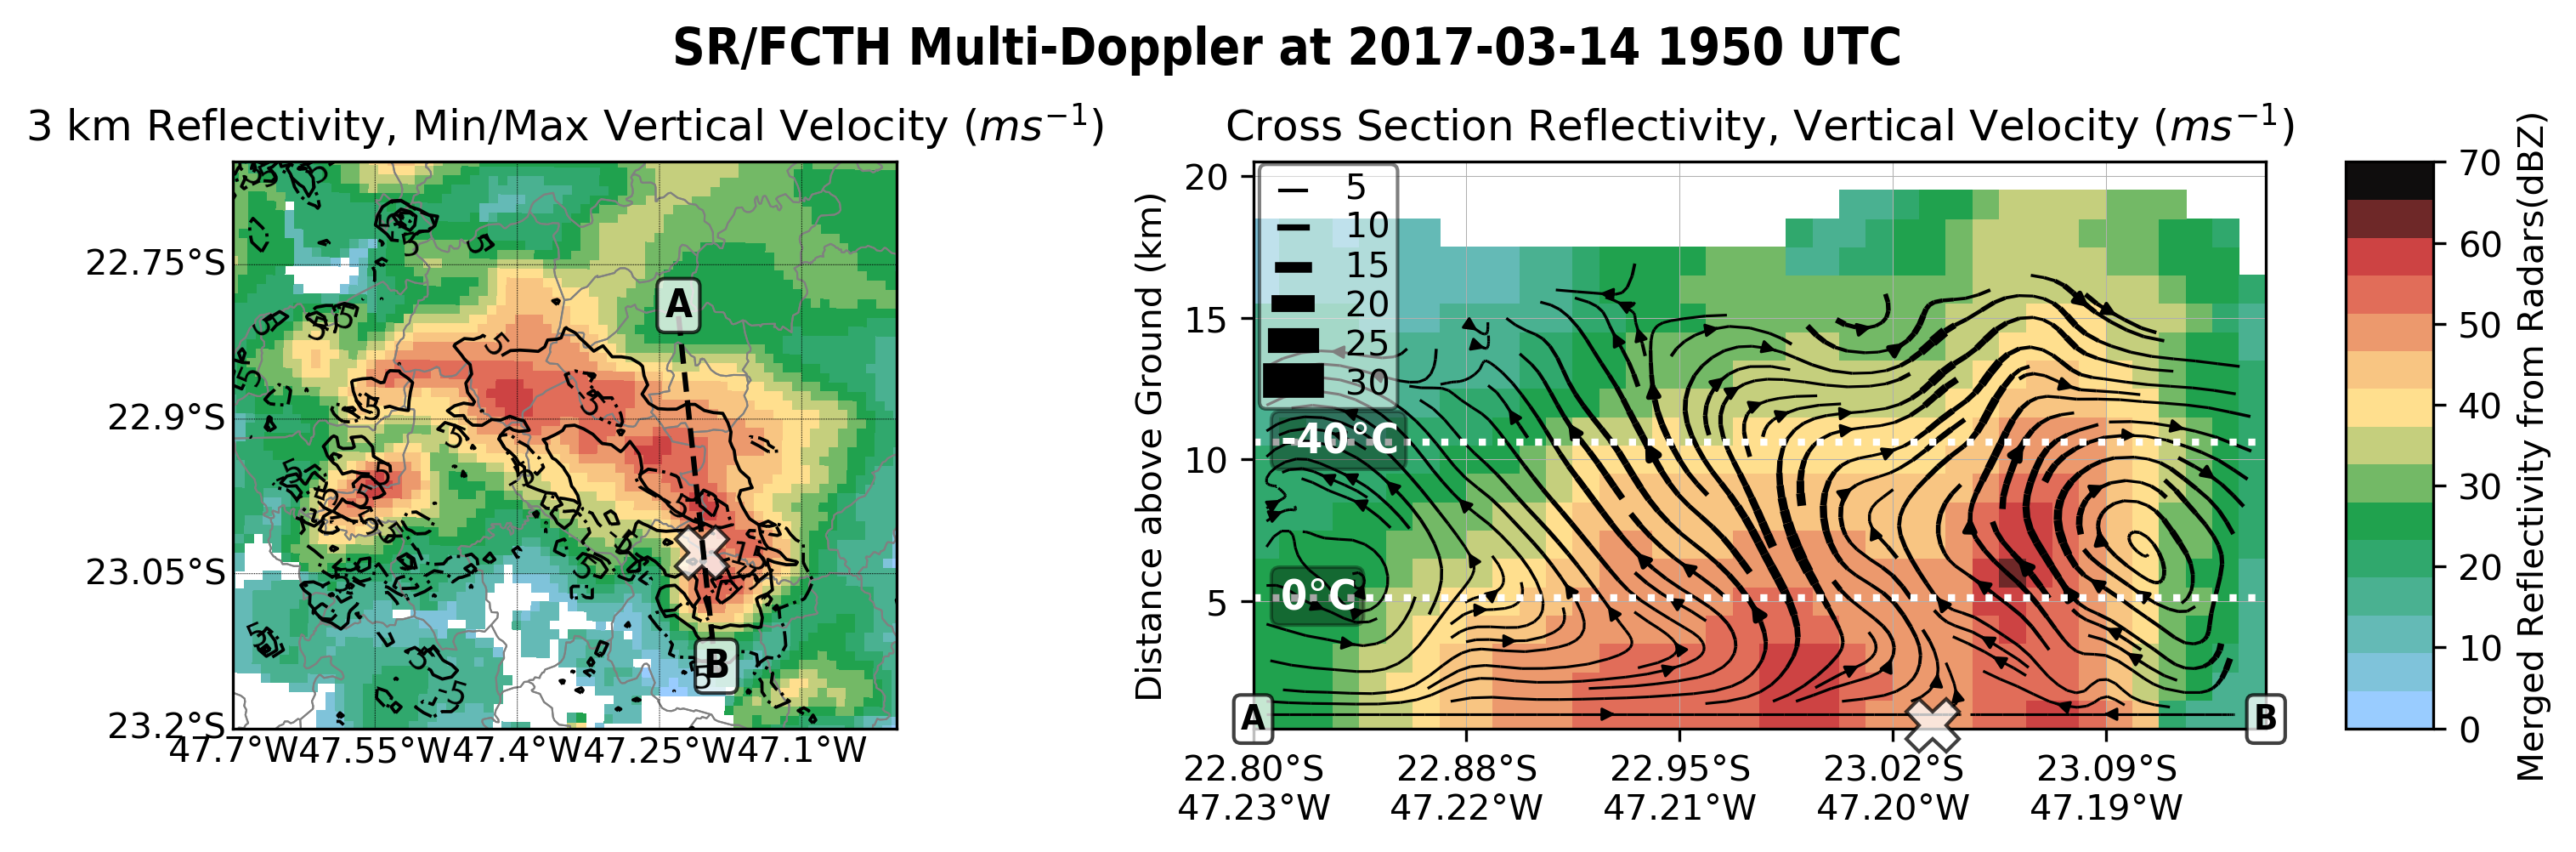
\includegraphics[width=\columnwidth]{../MultiDoppler_Processing/figures/SR-FCTH 2017-03-14 1950 UTC.png} \\
	\vspace{-5pt}
	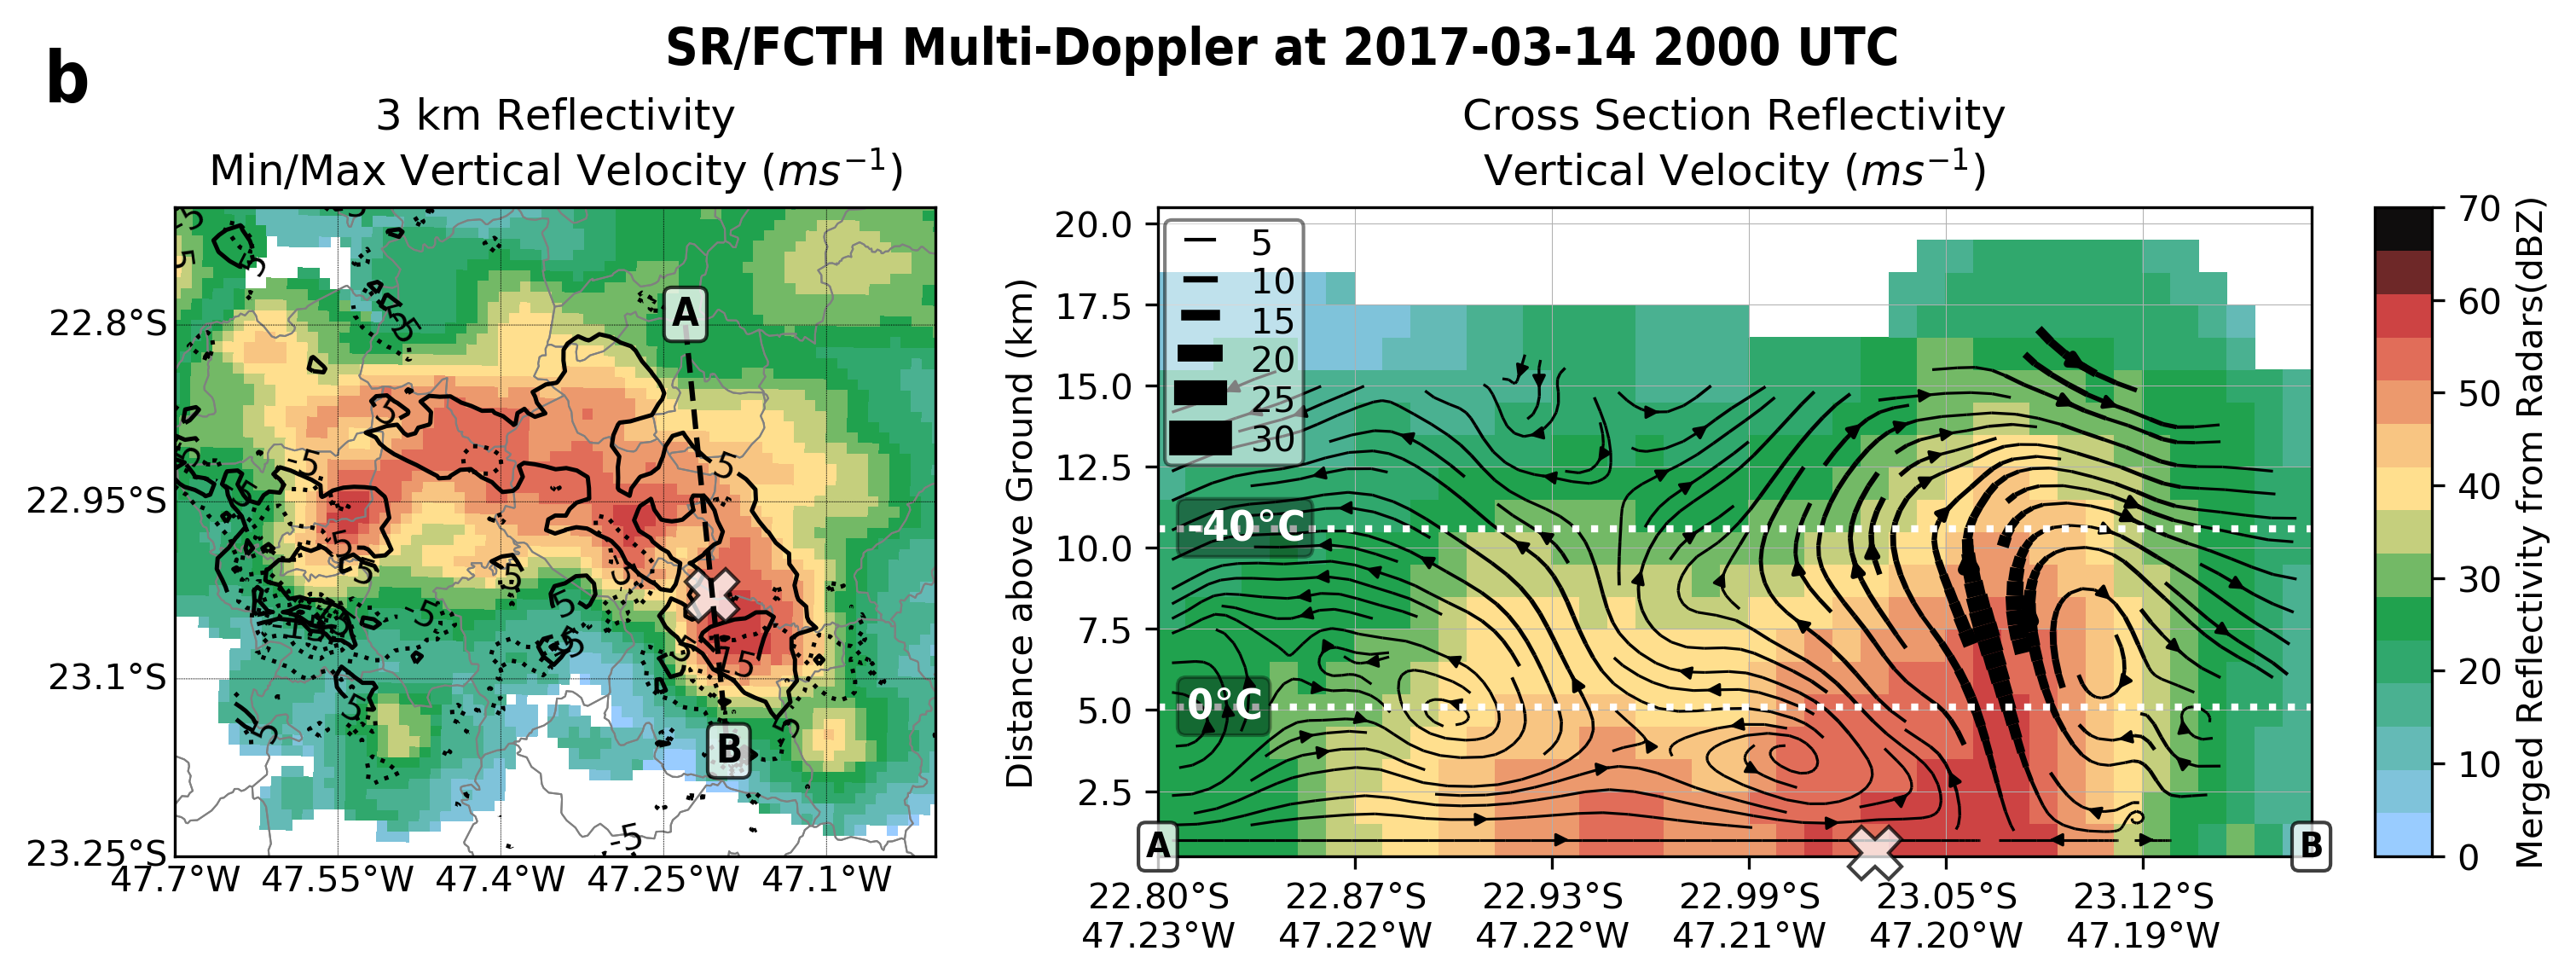
\includegraphics[width=\columnwidth]{../MultiDoppler_Processing/figures/SR-FCTH 2017-03-14 2000 UTC.png} \\
	\legend{Fonte: Produzido pela autora.}
\end{figure}

\subsection{Caso de 2017-11-15}

\subsubsection{Ambiente Sinótico e Termodinâmico}\label{sinotica_20171115}

Diferentemente do caso anterior, o caso de 2017-11-15 não teve condições sinóticas favoráveis. Mesmo com a Zona de Convergência do Atlântico Sul (ZCAS) localizada à norte do estado de São Paulo em fase de desconfiguração, a subsidência na região se manteve durante o dia: às 1200 UTC, a radiossondagem (\autoref{sondagem_20171115} mostra uma camada seca acima de $750\:hPa$, com baixo cisalhamento do vento e CAPE nulo, condição similar ao resto do estado (Figuras\autoref{era5_2017111512_jets} e\autoref{era5_2017111512_cape}); às 1800 UTC (Figura\autoref{era5_2017111518_cape}), o CAPE aumenta, mas ainda é baixo (entre 0 e $1000\:J\:kg^{-1}$), com um pouco de cisalhamento entre 1000 e $500\:hPa$ (até 5 nós). Ainda assim, as imagens de satélite mostram pequenos sistemas convectivos espalhados pelo centro-norte do estado se formando às 1800 (Figura\autoref{goes16_sp_20171115_1}) e 2100 UTC (Figura\autoref{goes16_sp_20171115_2}), com topos de nuvem de até $-60\:^{\circ}C$ de temperatura de brilho, incluindo o sistema que causou queda de granizo em Indaiatuba.

\begin{figure}[hp]
	\begin{center}
		\caption{Campos da reanálise do ERA5 em 2017-11-15: Pressão ao nível médio do mar, espessura entre $1000$ e $500\:hPa$ e velocidade do vento em $250\:hPa$ às 1200 UTC (a); altura geopotencial em $850\:hPa$, cisalhamento do vento entre $1000$ e $500\:hPa$ e CAPE em superfície às 1200 UTC (b) e 1800 UTC (c)} 
		\label{era5_20171115_main}
		\subfloat[]{\includegraphics[width=0.5\columnwidth]{../Reanalysis_Processing/figures/ERA5_SA_sfc-jets_201711151200.png}
			\label{era5_2017111512_jets}}
		\subfloat[]{\includegraphics[width=0.5\columnwidth]{../Reanalysis_Processing/figures/ERA5_SA_cape-shear_2017111512.png}
			\label{era5_2017111512_cape}} \\
		\subfloat[]{\includegraphics[width=0.5\columnwidth]{../Reanalysis_Processing/figures/ERA5_SP-BR_cape-shear_2017111518.png}
			\label{era5_2017111518_cape}} \\
		\legend{Fonte: Produzido pela autora.}
	\end{center}
\end{figure}

\begin{figure}[hp]
	\begin{center}
		\caption{Plotagem Skew-T Log-P da radiossondagem do Campo de Marte (SP) com hodógrafa do vento e índices CAPE e CIN em 2017-11-15 1200 UTC.} 
		\label{sondagem_20171115}
		%		\setcaptionmargin{1cm}
		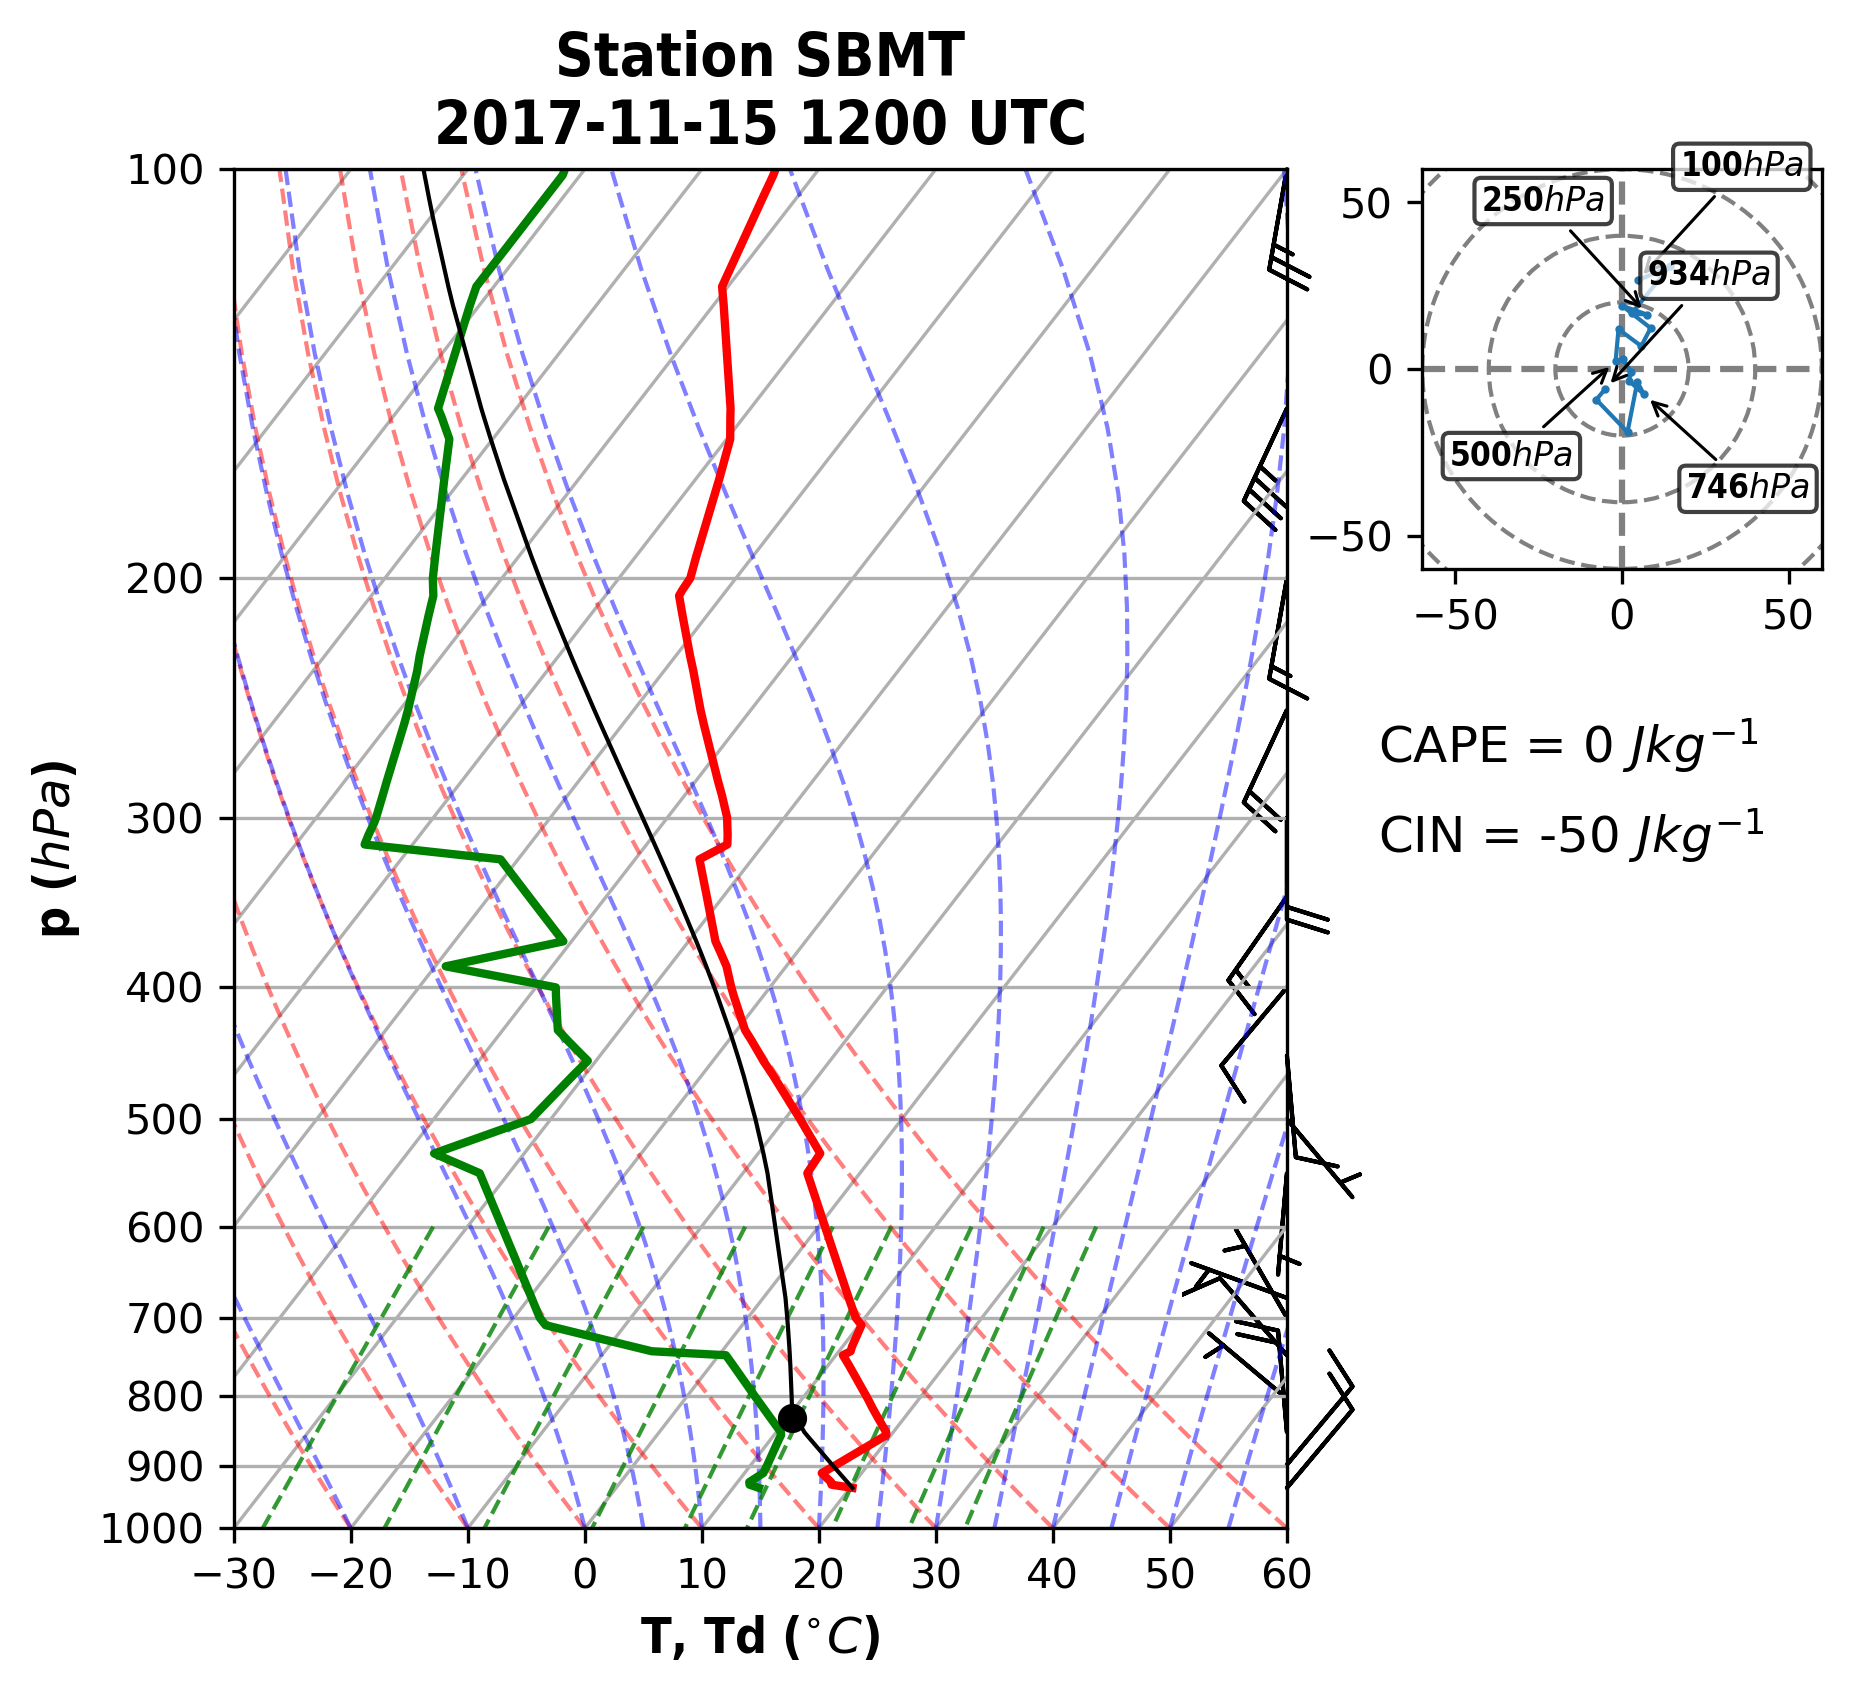
\includegraphics[width=0.75\columnwidth]{../Sounding_Processing/figures/sounding_SBMT2017111512UTC.png}
		\legend{Fonte: Produzido pela autora.}
	\end{center}
\end{figure}

%\begin{figure}[htb]
%	\begin{center}
%		\caption{Imagem de satélite do canal 13 do GOES-16 mostrando a temperatura de brilho do topo das nuvens na América do Sul em 2017-11-15 1800 UTC.} 
%		\label{goes16_sa_20171115}
%		%		\setcaptionmargin{1cm}
%		\includegraphics[width=0.75\columnwidth]{../Satellite_Processing/figures/Band_13/GOES16_B13_SA_SD201711151800.png}
%		\legend{Fonte: Produzido pela autora.}
%	\end{center}
%\end{figure}


\begin{figure}[hp]
	\begin{center}
		\caption{Imagem de satélite do canal 13 do GOES-16 mostrando a temperatura de brilho do topo das nuvens no estado de São Paulo em 2017-11-15 1800 (a) e 2100 UTC (b).} 
		\label{goes16_sp_20171115}
		\subfloat[]{\includegraphics[width=0.5\columnwidth]{../Satellite_Processing/figures/Band_13/GOES16_B13_SP-BR_SD201711151800.png}
			\label{goes16_sp_20171115_1}}
		\subfloat[]{\includegraphics[width=0.5\columnwidth]{../Satellite_Processing/figures/Band_13/GOES16_B13_SP-BR_SD201711152100.png}
			\label{goes16_sp_20171115_2}} \\
		\legend{Fonte: Produzido pela autora.}
	\end{center}
\end{figure}

\subsubsection{Eletrificação}\label{elec_20171115}

A \autoref{track_flashes_20171115} mostra a localização do sistema convectivo ao longo do ciclo de vida e dos \textit{flashes} associados a ele. Diferentemente do caso de 2017-03-14, já foi mostrado (\autoref{painel_ciclo}, \autoref{tabela_resumo_casos}) que o ciclo de vida desse sistema foi bem mais curto ($2,2\:h$) com baixa atividade elétrica (taxa máxima de 8 (3) $flashes\:min^{-1}$ IC (CG)) logo antes (depois, considerando apenas raios CG) da queda de granizo em Indaiatuba. O sistema passou por algumas cidades da RMC, sofrendo poucas fusões e separações (por ser um sistema pequeno e isolado). Boa parte dos \textit{flashes} (principalmente IC) ocorreram no sudoeste de Campinas e Indaiatuba, onde ocorreu a queda de granizo; em todo o ciclo de vida, cerca de 30\% dos \textit{flashes} foram CG, proporção maior do que no caso de 2017-03-14.

\begin{figure}[htb]
	\begin{center}
		\caption{Rastreamento (a) e localização dos \textit{flashes} IC e CG (b) do sistema convectivo responsável pela queda de granizo em Indaiatuba em 2017-11-15. Os triângulos pretos indicam a localização do \textit{hailpad}} 
		\label{track_flashes_20171115}
		%		\setcaptionmargin{1cm}
		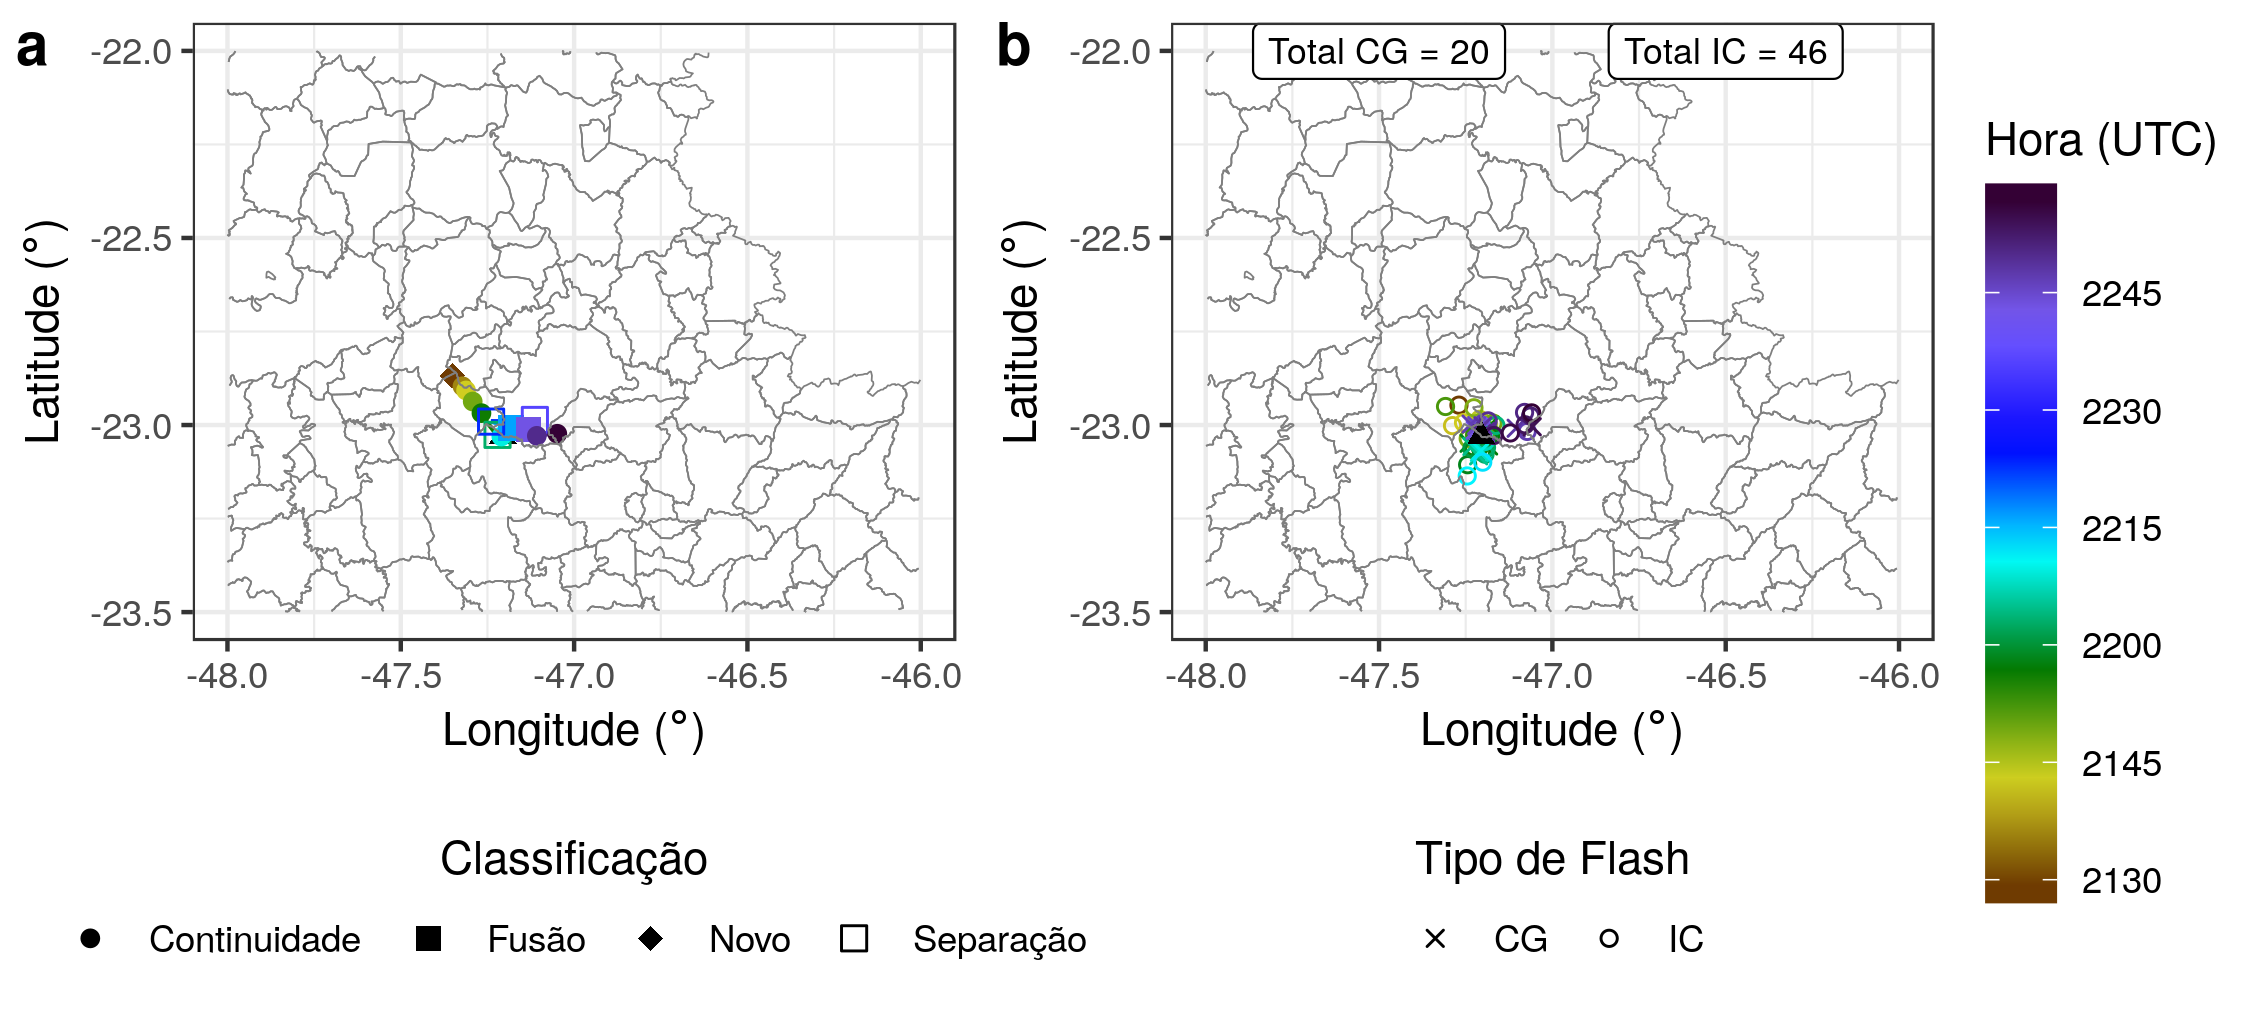
\includegraphics[width=\columnwidth]{../General_Processing/figures/track_flashes_20171115_ptbr.png}
		\legend{Fonte: Produzido pela autora.}
	\end{center}
\end{figure}

\subsubsection{Microfísica}\label{micro_20171115}

A \autoref{radar_20171115} mostra os campos de refletividade e variáveis polarimétricas refletividade diferencial, fase diferencial específica e coeficiente de correlação do radar da FCTH para o caso de 2017-11-15, quando houve queda de granizo em Indaiatuba; a \autoref{radar_derived_20171115} mostra a identificação de hidrometeoros e massas de água líquida e gelo calculadas a partir dos campos de radar. O núcleo convectivo responsável pela queda de granizo está embebido em um sistema que acabou de se separar de um sistema menor à noroeste. Esse núcleo é formado por uma região de refletividades acima de $50\:dBZ$ com cerca de $8\:km$ de extensão horizontal e $10\:km$ de extensão vertical (da superfície até a isoterma de $-40^{\circ}C$) (\autoref{radar_20171115}a). Entre a superfície e a isoterma de $0^{\circ}C$ observa-se refletividades acima de $60\:dBZ$ na localização do \textit{hailpad}, o que indica a presença de granizo ou chuva misturada com granizo - a refletividade diferencial (\autoref{radar_20171115}b) confirma isso, com valores entre 0 e $1\:dBZ$ nessa região.

\begin{figure}[hp]
	\centering
	\caption{Corte horizontal em $3\:km$ de altura e vertical entre os pontos A e B de campos do radar da FCTH em 2017-11-15 2150 UTC, quando houve queda de granizo em Indaiatuba: Refletividade corrigida (a) e diferencial (b), fase diferencial específica (c) e coeficiente de correlação (d). O 'x' indica a localização do \textit{hailpad} e as isotermas de $0$ e $-40^{\circ}C$ foram definidas a partir da radiossondagem de SMBT}
	\label{radar_20171115}
	\vspace{-5pt}
	\includegraphics[width=\columnwidth]{../Radar_Processing/figures/ppis/classification/FCTH Corrected Reflectivity 2017-11-15 2150 UTC.png} \\
	\vspace{-5pt}
	\includegraphics[width=\columnwidth]{../Radar_Processing/figures/ppis/classification/FCTH Differential Reflectivity 2017-11-15 2150 UTC.png} \\
	\vspace{-5pt}
	\includegraphics[width=\columnwidth]{../Radar_Processing/figures/ppis/classification/FCTH Specific Differential Phase 2017-11-15 2150 UTC.png} \\
	\vspace{-5pt}
	\includegraphics[width=\columnwidth]{../Radar_Processing/figures/ppis/classification/FCTH Cross Correlation Ratio 2017-11-15 2150 UTC.png} \\
	\legend{Fonte: Produzido pela autora.}
\end{figure}

\begin{figure}[htb]
	\centering
	\caption{Corte horizontal em $3\:km$ de altura e vertical entre os pontos A e B de campos derivados do radar da FCTH em 2017-11-15 2150 UTC, quando houve queda de granizo em Indaiatuba: Identificação de hidrometeoros (a) e massas de água líquida (b) e gelo (c). O 'x' indica a localização do \textit{hailpad} e as isotermas de $0$ e $-40^{\circ}C$ foram definidas a partir da radiossondagem de SMBT} 
	\label{radar_derived_20171115}
	\vspace{-5pt}
	\includegraphics[width=\columnwidth]{../Radar_Processing/figures/ppis/classification/FCTH Hydrometeor ID 2017-11-15 2150 UTC.png} \\
	\vspace{-5pt}
	\includegraphics[width=\columnwidth]{../Radar_Processing/figures/ppis/classification/FCTH Liquid Water Mass 2017-11-15 2150 UTC.png} \\
	\vspace{-5pt}
	\includegraphics[width=\columnwidth]{../Radar_Processing/figures/ppis/classification/FCTH Ice Water Mass 2017-11-15 2150 UTC.png} \\
	\legend{Fonte: Produzido pela autora.}
\end{figure}

A identificação de hidrometeoros no núcleo convectivo responsável pela queda de granizo (\autoref{radar_derived_20171115}a) novamente é similar ao campo de refletividade, classificando como granizo a região de refletividades acima de $50\:dBZ$, graupel de densidade alta entre 40 e $50\:dBZ$ e graupel de densidade baixa entre 30 e $40\:dBZ$. O problema está em regiões com refletividade abaixo de $30\:dBZ$, que são classificadas como cristais de gelo ou agregados mesmo abaixo da isoterma de $0^{\circ}C$ (em $\ang{23.03}S$, $\ang{47.17}W$, por exemplo, há cristais de gelo próximo à superfície. As variáveis polarimétricas indicam a presença de graupel), condição muito difícil de ser encontrada em nuvens frias de tempestades tropicais. Há uma maior concentração de massa de água líquida (cerca de $6\:gm^{-3}$, \autoref{radar_derived_20171115}b) próximo à superfície dentro do núcleo convectivo, extendendo-se até $7,5\:km$. A massa de gelo (\autoref{radar_derived_20171115}c), por outro lado, chega a concentrações muito mais altas ($30\:gm^{-3}$)  na mesma região, chegando a $12,5\:km$ de altura; essa alta concentração reforça a intensidade da queda de granizo observada no \textit{hailpad} (\autoref{tabela_resumo_casos}).

\subsubsection{Cinemática}\label{cinematica_20171115}

A \autoref{doppler_20171115} mostra os campos de refletividade mesclada e velocidade do vento derivado por Multi-Doppler usando a combinação dos radares de São Roque, FCTH e XPOL, para o caso de 2017-11-15, quando houve queda de granizo em Cosmópolis. O sistema convectivo responsável pelo evento mostra um núcleo isolado de refletividade acima de $40\:dBZ$ que se separa entre 2140 (\autoref{doppler_20171115}a) e 2150 UTC (\autoref{doppler_20171115}b), sendo que o núcleo mais intenso é localizado próximo ao \textit{hailpad}. Esse núcleo tem $15\:km$ de extensão vertical, com refletividades próximas a $55\:dBZ$ entre as isotermas de 0 e $-40^{\circ}C$ (\autoref{doppler_20171115}a) e acima de $60\:dBZ$ abaixo da isoterma de $0^{\circ}C$ (\autoref{doppler_20171115}b), indicando momentos distintos de formação e crescimento de hidrometeoros e subsequente precipitação. Antes da queda de granizo, uma região de corrente ascendente com velocidades de até $20\:ms^{-1}$ está associada ao núcleo convectivo, com um escoamento ascendente entre 5 e $13\:km$ de altura, divergência no topo e um escoamento descendente intenso (até $10\:ms^{-1}$) fora do núcleo, além de uma corrente descendente mais fraca dentro do núcleo. Dez minutos depois, a corrente ascendente (descendente) enfraquece (é fortalecida) dentro do núcleo convectivo, com um gradiente intenso (cerca de $5\:ms^{-1}km^{-1}$) entre as isotermas de 0 e $-40^{\circ}C$. Próximo à localização do \textit{hailpad}, a corrente descendente da isoterma de $0^{\circ}C$ à superfície e a refletividade de até $70\:dBZ$ próximo à superfície indicam intensa precipitação de hidrometeoros, incluindo chuva e granizos maiores (comparado ao caso de 2017-03-14), como observado pelo \textit{hailpad} (\autoref{tabela_resumo_casos}).

\begin{figure}[htb]
	\centering
	\caption{Corte horizontal em $3\:km$ de altura e vertical entre os pontos A e B de refletividade e velocidade do vento (correntes ascendentes e descendentes máximas no painel da esquerda, escoamento no painel da direita) derivado por Multi-Doppler em 2017-11-15 às 2140 (a) e 2150 UTC (b), quando houve queda de granizo em Cosmópolis. O 'x' indica a localização do \textit{hailpad} e as isotermas de $0$ e $-40^{\circ}C$ foram definidas a partir da radiossondagem de SMBT} 
	\label{doppler_20171115}
	\vspace{-5pt}
	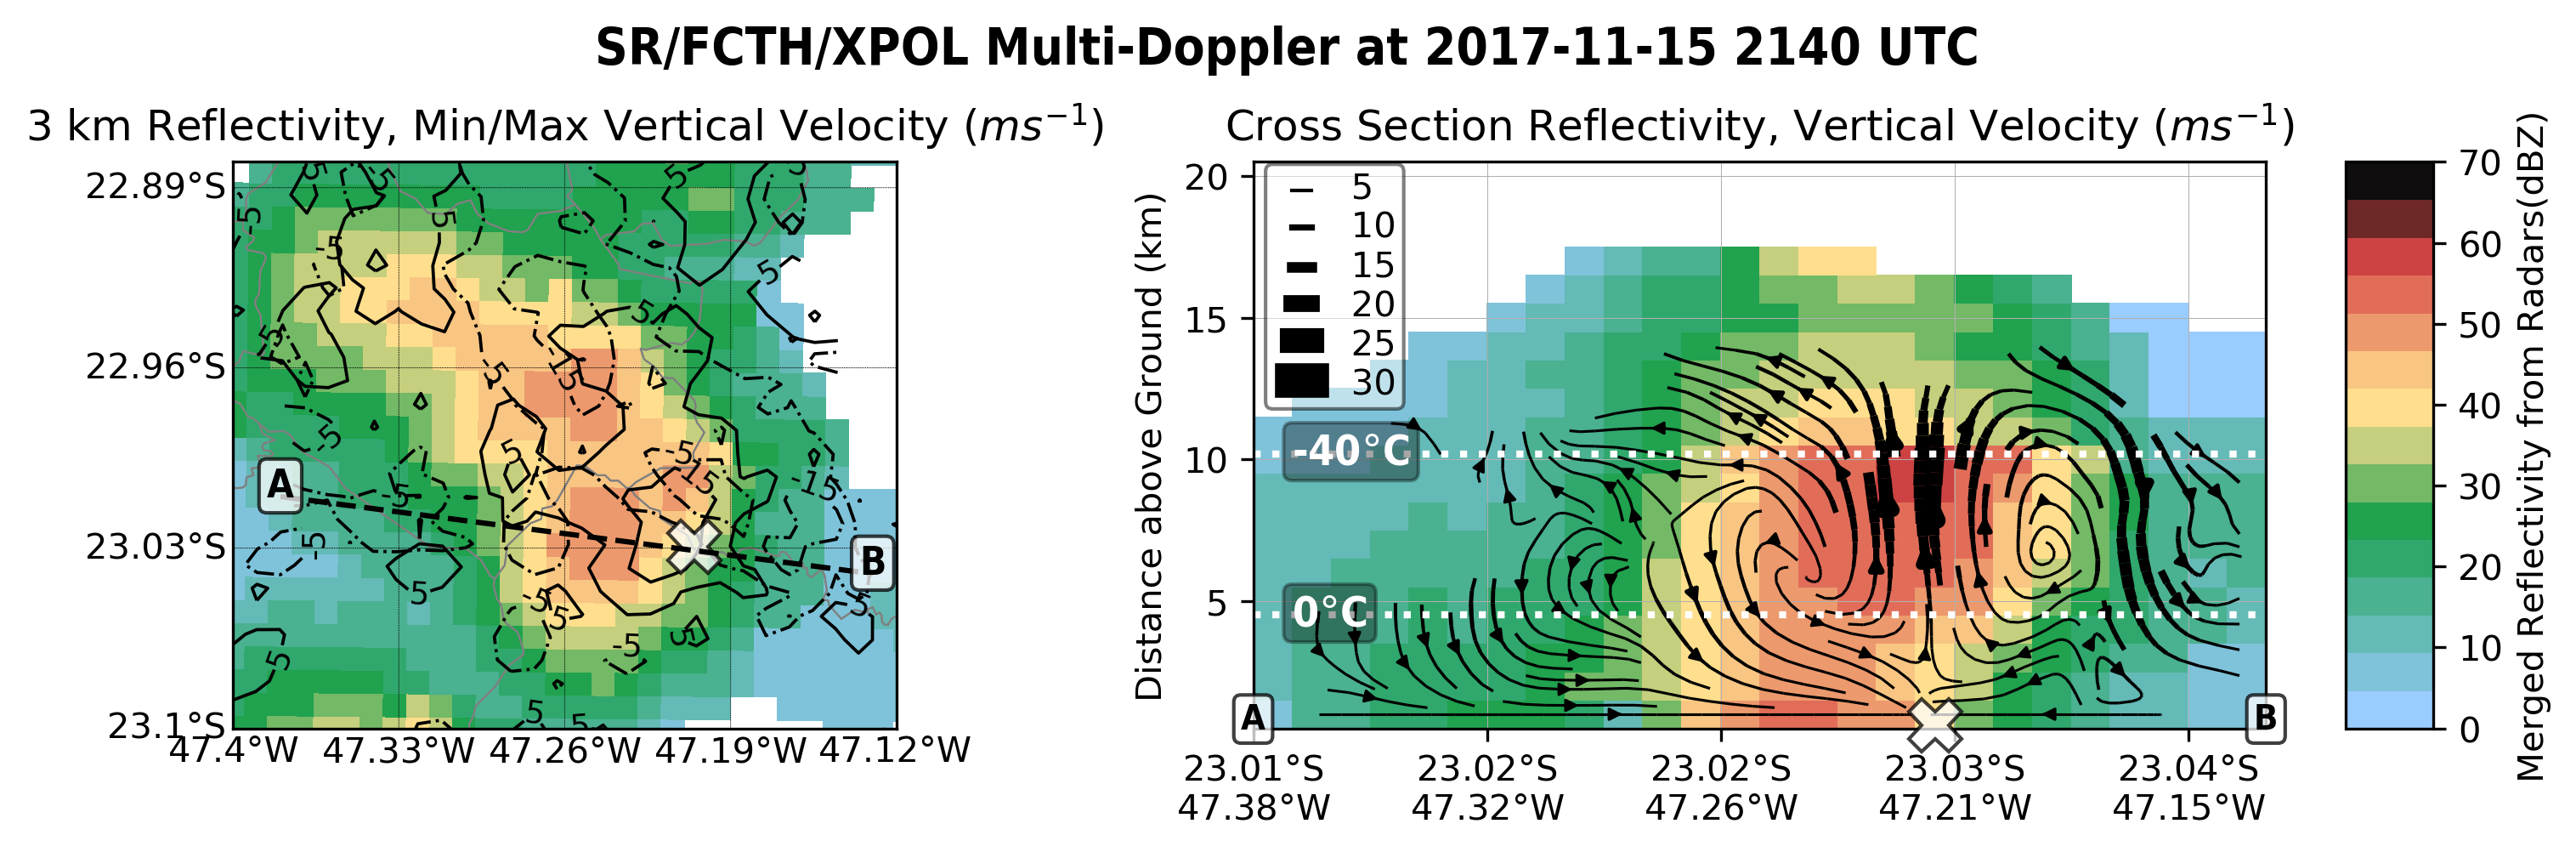
\includegraphics[width=\columnwidth]{../MultiDoppler_Processing/figures/SR-FCTH-XPOL 2017-11-15 2140 UTC.png} \\
	\vspace{-5pt}
	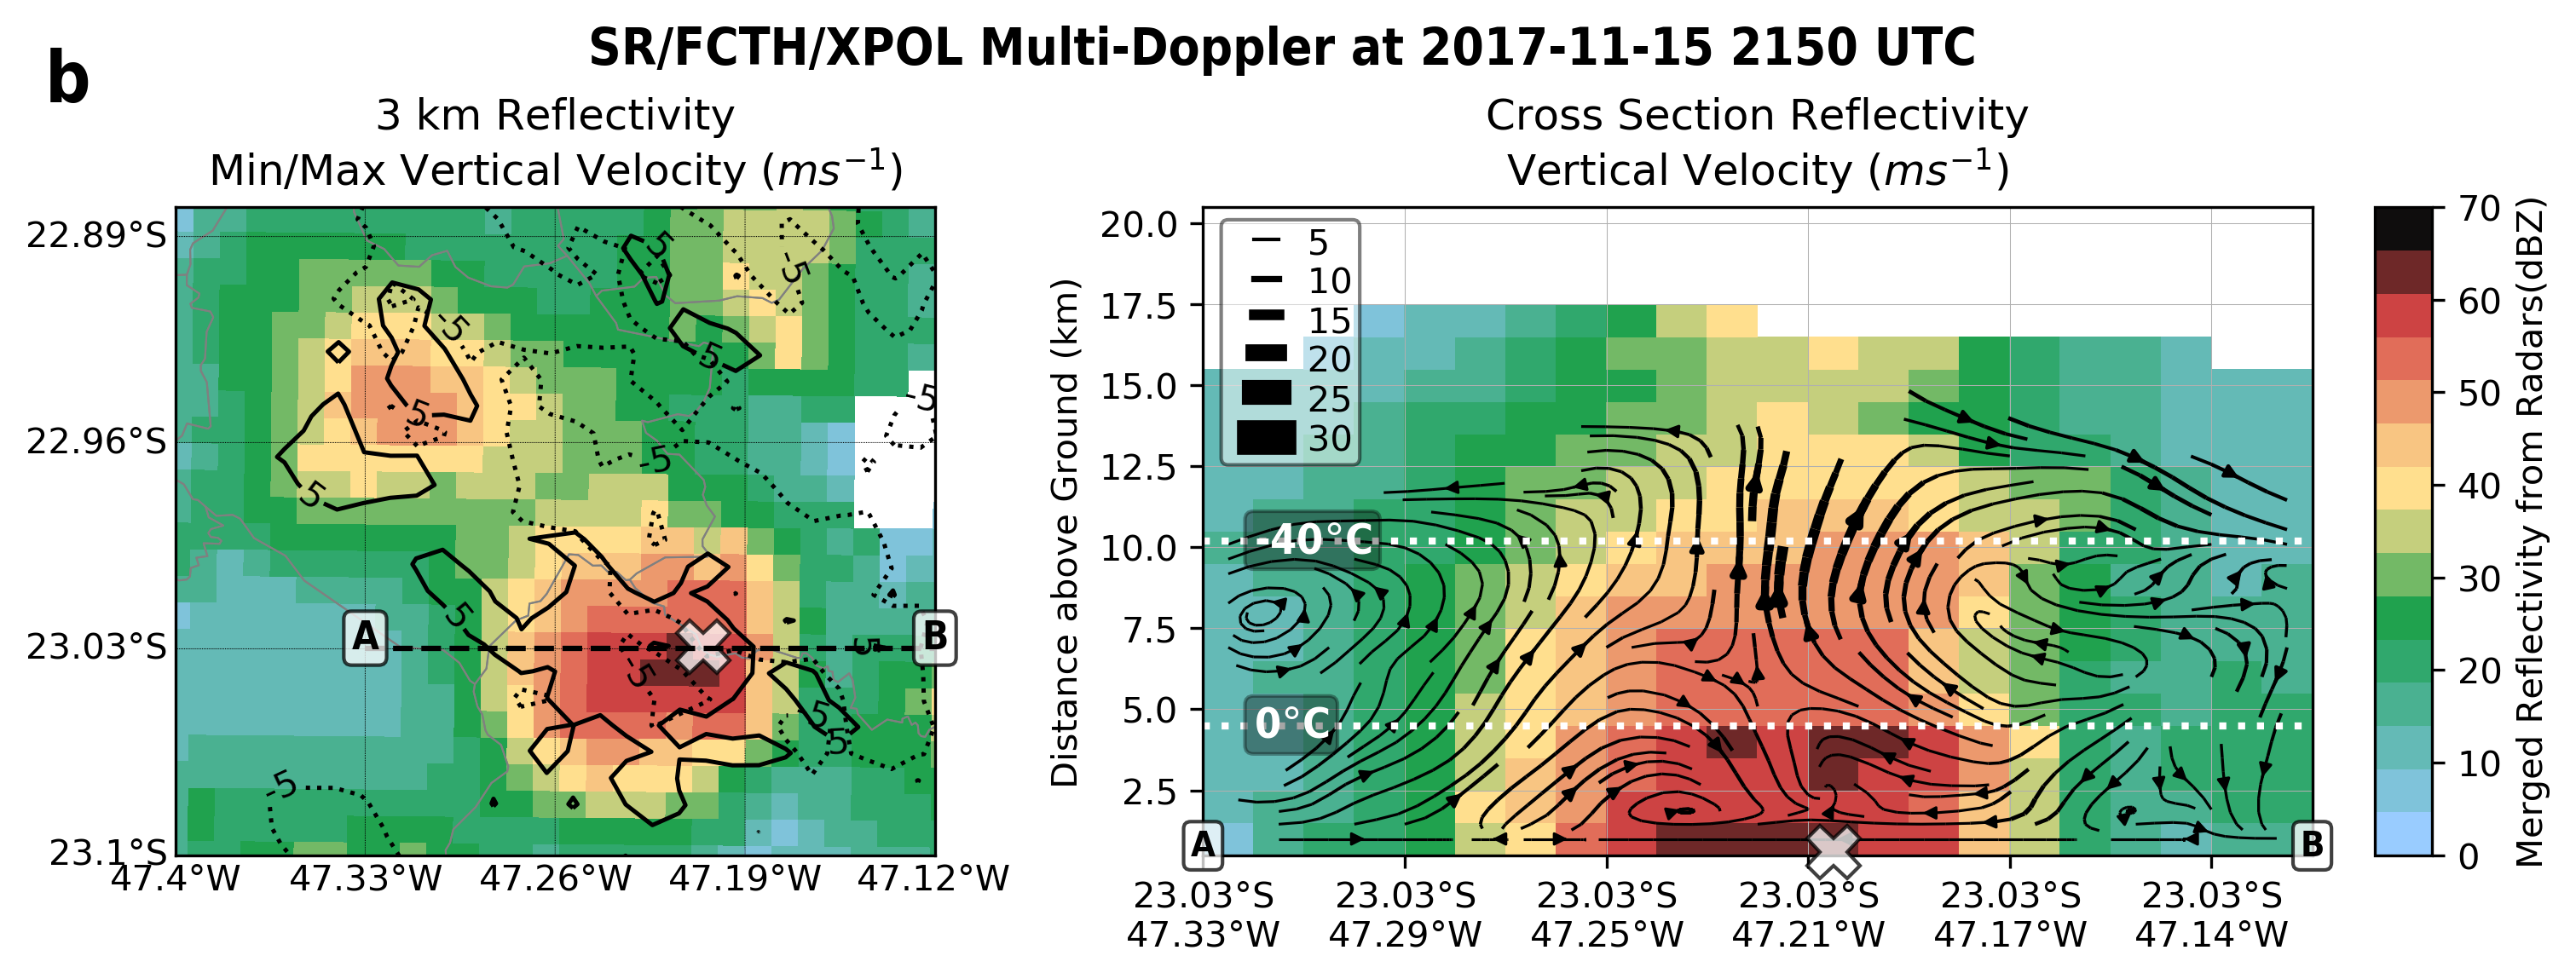
\includegraphics[width=\columnwidth]{../MultiDoppler_Processing/figures/SR-FCTH-XPOL 2017-11-15 2150 UTC.png} \\
	\legend{Fonte: Produzido pela autora.}
\end{figure}
